\documentclass[10pt, paper=8.5in:11in,pagesize=auto,openright,titlepage,cleardoublepage=empty, headinclude,twoside]{scrbook}

%\areaset[0mm]{5.5in}{9in} 
%  Syntax: \areaset[binding_correction]{textwidth}{textheight}

\usepackage{subfig}

\usepackage[eulerchapternumbers,
subfig,
beramono,
pdfspacing
,dottedtoc
]{classicthesis}

%altermundos tkz-euclide

% use axiom
% M123 book

\usepackage{arsclassica}
\usepackage{xfrac}

\areaset[5mm]{5.5in}{9in} 
\usepackage{verbatim}
\usepackage{varioref}
\usepackage{graphicx}
\usepackage{pdfpages}
\usepackage{chngpage}
\usepackage{amsmath,amssymb} 
\usepackage{amsthm,latexsym}   
\usepackage{harpoon}
%\usepackage{hyperref}
\usepackage{framed}
\usepackage{textcomp}
\usepackage{makeidx}
%\usepackage{heiroglf}
%\usepackage[dvipsnames]{color}
\usepackage{rotating}
\usepackage{multirow}

% tikz settings

\usepackage{pgf,tikz}
\usetikzlibrary{positioning,shadows,backgrounds}
\usetikzlibrary{arrows}
\usetikzlibrary{decorations.markings}
\tikzset{
  big arrow/.style={
    decoration={markings,
    mark=at position 0.01 with {\arrow[scale=2, #1]{<}};,
    mark=at position 1 with {\arrow[scale=2, #1]{>}}
    },
       postaction={decorate},
    shorten >=0.4pt},
  big arrow/.default=black}


\usepackage{xcolor}
\definecolor{shadecolor}{rgb}{0.75,0.75,0.75}
\usepackage{color}

\usepackage{enumitem}
\usepackage[framemethod=TikZ]{mdframed}


\usepackage{multicol}
\usepackage{multirow,colortbl}

\usepackage{mathtools}
\usepackage{enumitem}

%\renewcommand*{\chapterpagestyle}{empty}

\newcommand{\HUGE}{\fontsize{45}{50}\selectfont}
\newcommand{\exercs}{\fontsize{30}{40}\selectfont}
\newcommand{\exertitle}{\fontsize{20}{40}\selectfont}

\pdfbookmark[1]{\contentsname}{tableofcontents}

%\markboth{\spacedlowsmallcaps{\contentsname}}{\spacedlowsmallcaps{\contentsname}}

\automark[section]{chapter}
\theoremstyle{plain}
\newtheorem{thm}{Theorem}%[section]
\newtheorem*{thmn}{Theorem}
\newtheorem*{conj}{Conjecture}
\newtheorem{prop}[thm]{Proposition}
\newtheorem{lemma}[thm]{Lemma}
\newtheorem{cor}[thm]{Corollary}
\newtheorem*{postn}{Postulate}
\newtheorem{const}{Construction}
\newtheorem*{quesn}{Question}
\newtheorem*{quesns}{Questions}
\newtheorem*{prob}{Problem}

\theoremstyle{definition}
\newtheorem{defn}[thm]{Definition}
\newtheorem{ex}[thm]{Example}
\newtheorem{hyp}[thm]{Hypothesis}
\newtheorem{ques}[thm]{Question}

\theoremstyle{remark}
\newtheorem{rem}{Remark}
\newtheorem*{remn}{Remark}
\newtheorem{rrule}[thm]{Rule}
\newtheorem*{rrulen}{Rule}
\newtheorem*{notn}{Note}







%%%%%%%%%%
% blue box with title bold and in-line
%%%%%%%%%%


%\newenvironment{bluebox}[1][]{%
%\begin{mdframed}[%
%	skipabove=\baselineskip plus 2pt minus 1pt,
%    skipbelow=\baselineskip plus 2pt minus 1pt,
%innertopmargin=4pt,
%innerleftmargin=4pt,
%innerrightmargin=4pt,
%linewidth=0.0pt,
%linecolor=blue!15,
%backgroundcolor=blue!15,
%userdefinedwidth=10.5cm,
%align=center,
%roundcorner=4pt
%]\noindent\textbf{#1}\qquad%
%}{%
%    \end{mdframed}
%}
%
%
%
%%%%%%%%%%%
%% blue box with title bold and separate line
%%%%%%%%%%%
%
%
%\newenvironment{titlebox}[1][]{%
%    \begin{mdframed}[%
%        frametitle={\large #1},
%        skipabove=\baselineskip plus 2pt minus 1pt,
%        skipbelow=\baselineskip plus 2pt minus 1pt,
%        linewidth=0.5pt,
%linecolor=blue!15,
%        frametitlebackgroundcolor=blue!15,
%backgroundcolor=blue!15,
%userdefinedwidth=10.5cm,
%align=center,
%roundcorner=4pt
%    ]%
%}{%
%    \end{mdframed}
%}


%%%%%%%%%%
% wide blue box with title bold and separate line
%%%%%%%%%%


%\newenvironment{widetitlebox}[1][]{%
%    \begin{mdframed}[%
%        frametitle={\large #1},
%        skipabove=\baselineskip plus 2pt minus 1pt,
%        skipbelow=\baselineskip plus 2pt minus 1pt,
%        linewidth=0.5pt,
%linecolor=blue!15,
%        frametitlebackgroundcolor=blue!15,
%backgroundcolor=blue!15,
%userdefinedwidth=14.5cm,
%align=center,
%roundcorner=4pt
%    ]%
%}{%
%    \end{mdframed}
%}
%
%
%%%%%%%%%%%
%% Exercises Heading
%%%%%%%%%%%
%
%\newcommand{\exercises}{{\color{halfgray}\exertitle \noindent Exercises\,\,}{\exercs\color{halfgray}\arabic{chapter}.\arabic{section}} {\color{blue!15}\leaders\hrule height .8ex depth \dimexpr-.8ex+0.8pt\relax\hfill
%\vspace{3mm}} }
%
%%%%%%%%%%%
%% fancy example style
%%%%%%%%%%%
%
%
%\theoremstyle{definition}
%\newtheorem{exinn}{Example}[chapter]
%\newenvironment{example}
%  {\clubpenalty=10000
%   \begin{exinn}%
%   \mbox{}%
%   {\color{blue!15}\leaders\hrule height .8ex depth \dimexpr-.8ex+0.8pt\relax\hfill}%
%   \mbox{}\linebreak\ignorespaces}
%  {\par\kern2ex\color{blue!15}\hrule\end{exinn}}
%
%

%%%%%%%%%%
% On-Your-Own example 
%%%%%%%%%%
%
%\newtheoremstyle{noperiod}% name
%  {}%      Space above
%  {}%      Space below
%  {}%         Body font
%  {}%         Indent amount (empty = no indent, \parindent = para indent)
%  {\bfseries}% Thm head font
%  {}%        Punctuation after thm head
%  {.5em}%     Space after thm head: " " = normal interword space;
%        %       \newline = linebreak
%  {}%         Thm head spec (can be left empty, meaning `normal')
%
%\theoremstyle{noperiod}
%\newtheorem*{noperiod}{On Your Own \ldots}
%\newenvironment{oyoe}
%  {\clubpenalty=10000
%   \begin{noperiod}%
%   \mbox{}%
%   {\color{blue!15}\leaders\hrule height .8ex depth \dimexpr-.8ex+0.8pt\relax\hfill}%
%   \mbox{}\linebreak\ignorespaces}
%  {\par\kern2ex\color{blue!15}\hrule\end{noperiod}}


%%%%%%%%%%
% Custom commands
%%%%%%%%%%



\newcommand{\norm}[1]{\left\Vert#1\right\Vert}
\newcommand{\abs}[1]{\left\vert#1\right\vert}
\newcommand{\ip}[1]{\left\langle#1\right\rangle}
\newcommand{\set}[1]{\left\{#1\right\}}
\newcommand{\divides}{|}
\newcommand{\notdivides}{\!\!\not\divides \,}

% Standard sets

\newcommand{\Real}{\mathbb R}
\newcommand{\Int}{\mathbb Z}
\newcommand{\Nat}{\mathbb N}
\newcommand{\Rat}{\mathbb Q}
\newcommand{\Com}{\mathbb C}




\newcommand{\am}{_A\underline{\mbox{Mod}}}
\newcommand{\bm}{_B\underline{\mbox{Mod}}}
\newcommand{\bmo}{_{B^\circ}\underline{\mbox{Mod}}}
\newcommand{\To}{\longrightarrow}
\newcommand{\Hom}{\mbox{Hom}}
\newcommand{\ra}{\rightarrow}
\newcommand{\bds}{\begin{doublespace}}
\newcommand{\eds}{\end{doublespace}}
\newcommand{\mca}{\mathcal{A}}
\newcommand{\mcb}{\mathcal{B}}
\newcommand{\mcc}{\mathcal{C}}
\renewcommand{\phi}{\varphi}

\newcommand{\inv}[1]{{#1}^{-1}}
\newcommand{\da}[1]{(dx_{#1})_a}
\newcommand{\di}{\partial_i}
\renewcommand{\dj}{\partial_j}
\newcommand{\xTo}[1]{\xrightarrow{#1}}
\newcommand{\xMapsto}[1]{\xmapsto{#1}}
\newcommand{\dk}{\partial_k}
\newcommand{\bdy}{\partial}
\newcommand{\lcm}{\mathrm{lcm}}
\newcommand{\pstr}[1]{{\bf p}[#1]}
\newcommand{\psp}{\bf{p}}
\newcommand{\Aut}{\mathbb{A}}
\newcommand{\plo}{p\mathcal{L}}
\newcommand{\pls}{p\mathbb{S}}
\newcommand{\ls}{\mathbb{S}}
\newcommand{\cat}[1]{\textbf{\mbox{#1}}}

% high-light text, lists

%\newcommand{\hl}[1]{\colorbox{blue!15}{#1}}







\newcommand{\be}{\begin{enumerate}}
\newcommand{\ee}{\end{enumerate}}

\newcommand{\bal}{\begin{enumerate}[label=\textbf{\alph*.}]}
\newcommand{\eal}{\end{enumerate}}

\newcommand{\bexer}{\begin{enumerate}[label=\textbf{\large\arabic*.}\,\,]\itemsep=5mm}
\newcommand{\eexer}{\end{enumerate}}

\newcommand{\btc}{\begin{multicols}{2}}
\newcommand{\etc}{\end{multicols}}

\newcommand{\bmc}[1]{\begin{multicols}{#1}}

\newcommand{\dirns}[1]{\noindent \emph{#1}}

% Calculus

\newcommand{\deriv}[2]{\frac{\partial#1}{\partial x_#2}}
\newcommand{\vd}[2]{\frac{\partial#1}{\partial#2}}
\newcommand{\ddx}[1]{\frac{\partial#1}{\partial x}}
\newcommand{\ddy}[1]{\frac{\partial#1}{\partial y}}
\newcommand{\ddt}[1]{\frac{d#1}{dt}}

\newcommand{\Q}[1]{Q_{#1}^{(r)}}
\newcommand{\F}[1]{F_{#1}S\mathbb{A}_{r}}
\newcommand{\Out}{Out(F_n)}


% Canonical basis for R^3

\newcommand{\ivect}{\hat{\imath}}
\newcommand{\jvect}{\hat{\jmath}}
\newcommand{\kvect}{\hat{k}}



% Geometry

\newcommand{\ray}[1]{\overrightarrow{#1}}
\newcommand{\geoline}[1]{\overleftrightarrow{#1}}
\newcommand{\lineseg}[1]{\overline{#1}}
\newcommand{\arc}[1]{\wideparen{#1}}



%%%%%
%%  Number line tricks in tikz.  From User "Altermundus" at tex.se
%%%%%

%%%%%%%%%
%%%%%%%%%       Uncomment this for color version
%%%%%%%%%
%\newcommand{\mynumberline}[3]{%
%\begin{tikzpicture}[out=45,in=135,relative,>=stealth]
%\draw[<->] (#1-1,0)--(#2+1,0);
%\foreach \x in {\number\numexpr#1\relax,...,\number\numexpr#2\relax}  
%\draw[shift={(\x,0)},color=black] (0pt,2pt) -- (0pt,-2pt) node[below] {\footnotesize $\x$};
%
%\pgfmathsetmacro{\End}{#2-1} 
% \foreach \i in {#1,...,\End}{%
%    (\i,0) to (\i+1,0)
%} ; 
%\end{tikzpicture}}
%
%\newcommand{\mynumberray}[3]{%
%\begin{tikzpicture}[out=45,in=135,relative,>=stealth]
%\draw[->] (#1,0)--(#2+1,0);
%\foreach \x in {\number\numexpr#1\relax,...,\number\numexpr#2\relax}  
%\draw[shift={(\x,0)},color=black] (0pt,2pt) -- (0pt,-2pt) node[below] {\footnotesize $\x$};
%
%\pgfmathsetmacro{\End}{#2-1} 
% \foreach \i in {#1,...,\End}{%
%    (\i,0) to (\i+1,0)
%} ; 
%\end{tikzpicture}}
%
%\newcommand{\mynumberlinewithpoint}[3]{%
%\begin{tikzpicture}[out=45,in=135,relative,>=stealth]
%\draw[<->] (#1-1,0)--(#2+1,0);
%\foreach \x in {#3}
%\fill [color=black] (\x,0) circle (2.25pt);
%\foreach \x in {\number\numexpr#1\relax,...,\number\numexpr#2\relax}  
%\draw[shift={(\x,0)},color=black] (0pt,2pt) -- (0pt,-2pt) node[below] {\footnotesize $\x$};
%
%\pgfmathsetmacro{\End}{#2-1} 
% \foreach \i in {#1,...,\End}{%
%    (\i,0) to (\i+1,0)
%} ; 
%\end{tikzpicture}}
%
%
%
%
%
%
%\newcommand{\mysquarecoordplane}[2]{%
%\begin{tikzpicture}[scale=.5, out=45,in=135,relative,>=stealth]
%\draw[<->] (#1-1,0)--(#2+1,0);
%\foreach \x in {\number\numexpr#1\relax,...,-1}  
%\draw[shift={(\x,0)},color=black] (0pt,2pt) -- (0pt,-2pt) node[below] {\tiny $\x$};
%
%\foreach \x in {1,...,\number\numexpr#2\relax}  
%\draw[shift={(\x,0)},color=black] (0pt,2pt) -- (0pt,-2pt) node[below] {\tiny $\x$};
%
%\pgfmathsetmacro{\End}{#2-1} 
% \foreach \i in {#1,...,\End}{%
%    (\i,0) to (\i+1,0)
%} ; 
%
%\draw[<->] (0,#1-1)--(0,#2+1);
%\foreach \x in {\number\numexpr#1\relax,...,-1}  
%\draw[shift={(0,\x)},color=black] (2pt,0pt) -- (-2pt,0pt) node[right] {\tiny $\x$};
%\foreach \x in {1,...,\number\numexpr#2\relax}  
%\draw[shift={(0,\x)},color=black] (2pt,0pt) -- (-2pt,0pt) node[right] {\tiny $\x$};
%\pgfmathsetmacro{\End}{#2-1} 
% \foreach \i in {#1,...,\End}{%
%    (0,\i) to (0,\i+1)
%} ;
%
%\end{tikzpicture}}
%
%
%
%
%
%
%\newcommand{\addsubnumlinetoright}[3]{%
%\begin{tikzpicture}[out=45,in=135,relative,>=stealth]
%\draw[<->] (#1-2,0)--(#2+2,0);
%\foreach \x in {\number\numexpr#1-1\relax,...,\number\numexpr#2+1\relax}  
%\draw[shift={(\x,0)},color=black] (0pt,2pt) -- (0pt,-2pt) node[below] {\footnotesize $\x$};
%\fill (#1,0) circle (2pt);
%\fill (#2,0) circle (2pt);
%
%\pgfmathsetmacro{\End}{#2-1} 
% \draw[#3,shorten >=2pt]
% \foreach \i in {#1,...,\End}{%
%    (\i,0) to (\i+1,0)
%} ; 
%\node[color=Red] at (#2,-0.75) {\small End};
%\node[color=Green] at (#1,-0.75) {\small Start};
% \pgfmathsetmacro{\xtxt}{(#1+#2)/2}
%\node at (\xtxt,0.5) {\small Hop \number\numexpr#2-#1\relax\ units to the \emph{right}};
%\end{tikzpicture}}
%
%
%
%
%\newcommand{\symmnumbline}[3]{%
%\begin{tikzpicture}[out=45,in=135,relative,>=stealth]
%\draw[<->] (#1-2,0)--(#2+2,0);
%\foreach \x in {\number\numexpr#1-1\relax,...,\number\numexpr#2+1\relax}  
%\draw[shift={(\x,0)},color=black] (0pt,2pt) -- (0pt,-2pt) node[below] {\footnotesize $\x$};
%%\fill (#1,0) circle (2pt);
%%\fill (#2,0) circle (2pt);
%
%\pgfmathsetmacro{\Start}{#1-1} 
% \draw[#3,shorten >=2pt]
% \foreach \i in {\Start,...,-1}{%
%    (\i,0) to (-\i,0)
%} ; 
%
%\end{tikzpicture}}
%
%
%
%\newcommand{\disttozeronl}[3]{%
%\begin{tikzpicture}[out=45,in=135,relative,>=stealth]
%\draw[<->] (-3,0)--(3,0);
%\foreach \x in {\number\numexpr-3\relax,...,\number\numexpr3\relax}  
%\draw[shift={(\x,0)},color=black] (0pt,2pt) -- (0pt,-2pt) node[below] {\footnotesize $\x$};
%%\fill (1,0) circle (2pt);
%\fill (0,0) circle (2pt);
%
%\pgfmathsetmacro{\End}{#1+#2-1} 
% \draw[#3,shorten >=0pt]
% \foreach \i in {1}{%
%    (\i-1,0) to (\i,0)
%} ; 
%\end{tikzpicture}}
%
%
%\newcommand{\myaddsubnumlinetoright}[3]{%
%\begin{tikzpicture}[out=45,in=135,relative,>=stealth]
%\draw[<->] (#1-2,0)--(#1+#2+2,0);
%\foreach \x in {\number\numexpr#1-1\relax,...,\number\numexpr#1+#2+1\relax}  
%\draw[shift={(\x,0)},color=black] (0pt,2pt) -- (0pt,-2pt) node[below] {\footnotesize $\x$};
%\fill (#1,0) circle (2pt);
%\fill (#1+#2,0) circle (2pt);
%
%\pgfmathsetmacro{\End}{#1+#2-1} 
% \draw[#3,shorten >=2pt]
% \foreach \i in {#1,...,\End}{%
%    (\i,0) to (\i+1,0)
%} ; 
%\node[color=Red] at (#1+#2,-0.75) {\small End};
%\node[color=Green] at (#1,-0.75) {\small Start};
% \pgfmathsetmacro{\xtxt}{(#1+#1+#2)/2}
%\node at (\xtxt,0.5) {\small Hop \number\numexpr#2\relax\ units to the \emph{right}};
%\end{tikzpicture}}
%
%
%\newcommand{\addsubnumlinetoleft}[3]{%
%\begin{tikzpicture}[out=135,in=45,>=stealth]
%\draw[<->] (#2-2,0)--(#1+2,0);
%\foreach \x in {\number\numexpr#2-1\relax,...,\number\numexpr#1+1\relax}
%\draw[shift={(\x,0)},color=black] (0pt,2pt) -- (0pt,-2pt) node[below] {\footnotesize $\x$};
%\fill (#1,0) circle (2pt);
%\fill (#2,0) circle (2pt);
%
%\pgfmathsetmacro{\End}{#2+1} 
% \draw[#3,shorten >=2pt]
% \foreach \i in {#1,...,\End}{%
%    (\i,0) to  (\i-1,0)
%} ; 
%\node[color=Red] at (#2,-0.75) {\small End };
%\node[color=Green] at (#1,-0.75) {\small Start };
% \pgfmathsetmacro{\xtxt}{(#1+#2)/2}     
%\node at (\xtxt,0.5) {\small Hop \number\numexpr-#2+#1\relax\ units to the \emph{left}};
%\end{tikzpicture}} 







%%%%%%%%%%%%%%%%%%%%%%%%%%%%%%%%%%%%%%%%%%%%%%%%%%%%%%%%%%%%%%%%%%%%%%%%%%%
%%%%%%%%%%%%%%%%%%%%%%%%%%%%%%%%%%%%%%%%%%%%%%%%%%%%%%%%%%%%%%%%%%%%%%%%%%%
%%%%%%%%%%%%%%%%%%%%%%%%%%%%%%%%%%%%%%%%%%%%%%%%%%%%%%%%%%%%%%%%%%%%%%%%%%%
%%%%   Grayscale versions of highlight, boxes, examples, etc.          %%%%
%%%%%%%%%%%%%%%%%%%%%%%%%%%%%%%%%%%%%%%%%%%%%%%%%%%%%%%%%%%%%%%%%%%%%%%%%%%
%%%%%%%%%%%%%%%%%%%%%%%%%%%%%%%%%%%%%%%%%%%%%%%%%%%%%%%%%%%%%%%%%%%%%%%%%%%
%%%%%%%%%%%%%%%%%%%%%%%%%%%%%%%%%%%%%%%%%%%%%%%%%%%%%%%%%%%%%%%%%%%%%%%%%%%

% grayscale highlight

\newcommand{\hl}[1]{\colorbox{gray!40}{#1}}




\newcommand{\mynumberline}[3]{%
\begin{tikzpicture}[out=45,in=135,relative,>=stealth]
\draw[<->] (#1-1,0)--(#2+1,0);
\foreach \x in {\number\numexpr#1\relax,...,\number\numexpr#2\relax}  
\draw[shift={(\x,0)},color=black] (0pt,2pt) -- (0pt,-2pt) node[below] {\footnotesize $\x$};

\pgfmathsetmacro{\End}{#2-1} 
 \foreach \i in {#1,...,\End}{%
    (\i,0) to (\i+1,0)
} ; 
\end{tikzpicture}}

\newcommand{\mynumberray}[3]{%
\begin{tikzpicture}[out=45,in=135,relative,>=stealth]
\draw[->] (#1,0)--(#2+1,0);
\foreach \x in {\number\numexpr#1\relax,...,\number\numexpr#2\relax}  
\draw[shift={(\x,0)},color=black] (0pt,2pt) -- (0pt,-2pt) node[below] {\footnotesize $\x$};

\pgfmathsetmacro{\End}{#2-1} 
 \foreach \i in {#1,...,\End}{%
    (\i,0) to (\i+1,0)
} ; 
\end{tikzpicture}}

\newcommand{\mynumberlinewithpoint}[3]{%
\begin{tikzpicture}[out=45,in=135,relative,>=stealth]
\draw[<->] (#1-1,0)--(#2+1,0);
\foreach \x in {#3}
\fill [color=black] (\x,0) circle (2.25pt);
\foreach \x in {\number\numexpr#1\relax,...,\number\numexpr#2\relax}  
\draw[shift={(\x,0)},color=black] (0pt,2pt) -- (0pt,-2pt) node[below] {\footnotesize $\x$};

\pgfmathsetmacro{\End}{#2-1} 
 \foreach \i in {#1,...,\End}{%
    (\i,0) to (\i+1,0)
} ; 
\end{tikzpicture}}






\newcommand{\mysquarecoordplane}[2]{%
\begin{tikzpicture}[scale=.5, out=45,in=135,relative,>=stealth]
\draw[<->] (#1-1,0)--(#2+1,0);
\foreach \x in {\number\numexpr#1\relax,...,-1}  
\draw[shift={(\x,0)},color=black] (0pt,2pt) -- (0pt,-2pt) node[below] {\tiny $\x$};

\foreach \x in {1,...,\number\numexpr#2\relax}  
\draw[shift={(\x,0)},color=black] (0pt,2pt) -- (0pt,-2pt) node[below] {\tiny $\x$};

\pgfmathsetmacro{\End}{#2-1} 
 \foreach \i in {#1,...,\End}{%
    (\i,0) to (\i+1,0)
} ; 

\draw[<->] (0,#1-1)--(0,#2+1);
\foreach \x in {\number\numexpr#1\relax,...,-1}  
\draw[shift={(0,\x)},color=black] (2pt,0pt) -- (-2pt,0pt) node[right] {\tiny $\x$};
\foreach \x in {1,...,\number\numexpr#2\relax}  
\draw[shift={(0,\x)},color=black] (2pt,0pt) -- (-2pt,0pt) node[right] {\tiny $\x$};
\pgfmathsetmacro{\End}{#2-1} 
 \foreach \i in {#1,...,\End}{%
    (0,\i) to (0,\i+1)
} ;

\end{tikzpicture}}






\newcommand{\addsubnumlinetoright}[3]{%
\begin{tikzpicture}[out=45,in=135,relative,>=stealth]
\draw[<->] (#1-2,0)--(#2+2,0);
\foreach \x in {\number\numexpr#1-1\relax,...,\number\numexpr#2+1\relax}  
\draw[shift={(\x,0)},color=black] (0pt,2pt) -- (0pt,-2pt) node[below] {\footnotesize $\x$};
\fill (#1,0) circle (2pt);
\fill (#2,0) circle (2pt);

\pgfmathsetmacro{\End}{#2-1} 
 \draw[#3,shorten >=2pt,color=black]
 \foreach \i in {#1,...,\End}{%
    (\i,0) to (\i+1,0)
} ; 
\node[color=black] at (#2,-0.75) {\small End};
\node[color=black] at (#1,-0.75) {\small Start};
 \pgfmathsetmacro{\xtxt}{(#1+#2)/2}
\node at (\xtxt,0.5) {\small Hop \number\numexpr#2-#1\relax\ units to the \emph{right}};
\end{tikzpicture}}




\newcommand{\symmnumbline}[3]{%
\begin{tikzpicture}[out=45,in=135,relative,>=stealth]
\draw[<->] (#1-2,0)--(#2+2,0);
\foreach \x in {\number\numexpr#1-1\relax,...,\number\numexpr#2+1\relax}  
\draw[shift={(\x,0)},color=black] (0pt,2pt) -- (0pt,-2pt) node[below] {\footnotesize $\x$};
%\fill (#1,0) circle (2pt);
%\fill (#2,0) circle (2pt);

\pgfmathsetmacro{\Start}{#1-1} 
 \draw[#3,shorten >=2pt,color=black]
 \foreach \i in {\Start,...,-1}{%
    (\i,0) to (-\i,0)
} ; 

\end{tikzpicture}}



\newcommand{\disttozeronl}[3]{%
\begin{tikzpicture}[out=45,in=135,relative,>=stealth]
\draw[<->] (-3,0)--(3,0);
\foreach \x in {\number\numexpr-3\relax,...,\number\numexpr3\relax}  
\draw[shift={(\x,0)},color=black] (0pt,2pt) -- (0pt,-2pt) node[below] {\footnotesize $\x$};
%\fill (1,0) circle (2pt);
%\fill (0,0) circle (2pt);

\pgfmathsetmacro{\End}{#1+#2-1} 
 \draw[#3,shorten >=0pt,color=black]
 \foreach \i in {1}{%
    (\i-1,0) to (\i,0)
} ; 
\end{tikzpicture}}


\newcommand{\myaddsubnumlinetoright}[3]{%
\begin{tikzpicture}[out=45,in=135,relative,>=stealth]
\draw[<->] (#1-2,0)--(#1+#2+2,0);
\foreach \x in {\number\numexpr#1-1\relax,...,\number\numexpr#1+#2+1\relax}  
\draw[shift={(\x,0)},color=black] (0pt,2pt) -- (0pt,-2pt) node[below] {\footnotesize $\x$};
\fill (#1,0) circle (2pt);
\fill (#1+#2,0) circle (2pt);

\pgfmathsetmacro{\End}{#1+#2-1} 
 \draw[#3,shorten >=2pt,color=black]
 \foreach \i in {#1,...,\End}{%
    (\i,0) to (\i+1,0)
} ; 
\node[color=black] at (#1+#2,-0.75) {\small End};
\node[color=black] at (#1,-0.75) {\small Start};
 \pgfmathsetmacro{\xtxt}{(#1+#1+#2)/2}
\node at (\xtxt,0.5) {\small Hop  \number\numexpr#2\relax\ units to the \emph{right}};
\end{tikzpicture}}


\newcommand{\addsubnumlinetoleft}[3]{%
\begin{tikzpicture}[out=135,in=45,>=stealth]
\draw[<->] (#2-2,0)--(#1+2,0);
\foreach \x in {\number\numexpr#2-1\relax,...,\number\numexpr#1+1\relax}
\draw[shift={(\x,0)},color=black] (0pt,2pt) -- (0pt,-2pt) node[below] {\footnotesize $\x$};
\fill (#1,0) circle (2pt);
\fill (#2,0) circle (2pt);

\pgfmathsetmacro{\End}{#2+1} 
 \draw[#3,shorten >=2pt,color=black]
 \foreach \i in {#1,...,\End}{%
    (\i,0) to  (\i-1,0)
} ; 
\node[color=black] at (#2,-0.75) {\small End };
\node[color=black] at (#1,-0.75) {\small Start };
 \pgfmathsetmacro{\xtxt}{(#1+#2)/2}     
\node at (\xtxt,0.5) {\small Hop \number\numexpr-#2+#1\relax\ units to the \emph{left}};
\end{tikzpicture}} 















%%%%%%%%%%
% blue box with title bold and in-line
%%%%%%%%%%


\newenvironment{bluebox}[1][]{%
\begin{mdframed}[%
	skipabove=\baselineskip plus 2pt minus 1pt,
    skipbelow=\baselineskip plus 2pt minus 1pt,
innertopmargin=4pt,
innerleftmargin=4pt,
innerrightmargin=4pt,
linewidth=0.0pt,
linecolor=halfgray,
backgroundcolor=halfgray,
userdefinedwidth=10.5cm,
align=center,
roundcorner=4pt
]\noindent\textbf{#1}\qquad%
}{%
    \end{mdframed}
}



%%%%%%%%%%
% blue box with title bold and separate line
%%%%%%%%%%


\newenvironment{titlebox}[1][]{%
    \begin{mdframed}[%
        frametitle={\large #1},
        skipabove=\baselineskip plus 2pt minus 1pt,
        skipbelow=\baselineskip plus 2pt minus 1pt,
        linewidth=0.5pt,
linecolor=halfgray,
        frametitlebackgroundcolor=halfgray,
backgroundcolor=halfgray,
userdefinedwidth=10.5cm,
align=center,
roundcorner=4pt
    ]%
}{%
    \end{mdframed}
}


%%%%%%%%%%
% wide blue box with title bold and separate line
%%%%%%%%%%


\newenvironment{widetitlebox}[1][]{%
    \begin{mdframed}[%
        frametitle={\large #1},
        skipabove=\baselineskip plus 2pt minus 1pt,
        skipbelow=\baselineskip plus 2pt minus 1pt,
        linewidth=0.5pt,
linecolor=halfgray,
        frametitlebackgroundcolor=halfgray,
backgroundcolor=halfgray,
userdefinedwidth=14.5cm,
align=center,
roundcorner=4pt
    ]%
}{%
    \end{mdframed}
}


%%%%%%%%%%
% Exercises Heading
%%%%%%%%%%

\newcommand{\exercises}{\newpage{\color{halfgray}\exertitle \noindent Exercises\,\,}{\exercs\color{halfgray}\arabic{chapter}.\arabic{section}} {\color{halfgray}\leaders\hrule height .8ex depth \dimexpr-.8ex+0.8pt\relax\hfill
\vspace{3mm}} }

%%%%%%%%%%
% fancy example style
%%%%%%%%%%


\theoremstyle{definition}
\newtheorem{exinn}{Example}[section]
\newenvironment{example}
  {\clubpenalty=10000
   \begin{exinn}%
   \mbox{}%
   {\color{halfgray}\leaders\hrule height .8ex depth \dimexpr-.8ex+0.8pt\relax\hfill}%
   \mbox{}\linebreak\ignorespaces}
  {\par\kern2ex\color{halfgray}\hrule\end{exinn}}



%%%%%%%%%%
% On-Your-Own example 
%%%%%%%%%%

\newtheoremstyle{noperiod}% name
  {.5cm}%      Space above
  {.5cm}%      Space below
  {}%         Body font
  {}%         Indent amount (empty = no indent, \parindent = para indent)
  {\bfseries}% Thm head font
  {}%        Punctuation after thm head
  {.5em}%     Space after thm head: " " = normal interword space;
        %       \newline = linebreak
  {}%         Thm head spec (can be left empty, meaning `normal')

\theoremstyle{noperiod}
\newtheorem*{noperiod}{On Your Own \ldots}
\newenvironment{oyoe}
  {\clubpenalty=10000
   \begin{noperiod}%
   \mbox{}%
   {\color{halfgray}\leaders\hrule height .8ex depth \dimexpr-.8ex+0.8pt\relax\hfill}%
   \mbox{}\linebreak\ignorespaces}
  {\par\kern2ex\color{halfgray}\hrule\end{noperiod}}





\let\orgtheindex\theindex
\let\orgendtheindex\endtheindex
\def\theindex{%
	\def\twocolumn{\begin{multicols}{2}}%
	\def\onecolumn{}%
	\clearpage
	\orgtheindex
}
\def\endtheindex{%
	\end{multicols}%
	\orgendtheindex
}

\makeindex

\DeclareRobustCommand*{\arsclassica}{{\normalfont\sffamily ArsClassica}}
\DeclareRobustCommand*{\texlive}{\TeX{}~Live%
\index{texlive@\protect\TeX{}~Live}}




\newcommand{\myTitle}{Curriculum Guide}
\newcommand{\mySubTitle}{2022-2023 Edition}
\newcommand{\myLocation}{Indian Springs School}
%\newcommand{\myGroup}{Italian \TeX{} and \LaTeX{} User Group}
%\newcommand{\myUrl}{\url{http://www.guitex.org/}}
%\newcommand{\myTime}{2012, February}

\font\manual=manfnt
\def\dbend{{\manual\char127}} % dangerous bend sign

% ----------------------------------------------------------------
\begin{document}

\pagenumbering{roman}
\pagestyle{plain}






%******************************************************************
% Frontmatter
%******************************************************************

\frontmatter
\begin{titlepage}
\pdfbookmark{Titlepage}{Titlepage}
\changetext{}{}{}{((\paperwidth  - \textwidth) / 2) - \oddsidemargin - \hoffset - 1in}{}
\null\vfill
\begin{center}
\large
\sffamily




\includegraphics[width=10.75cm]{crest}

\vspace{10cm}

{\Huge{\myTitle}} \\

\bigskip

{\LARGE{\mySubTitle}} \\

\bigskip

\mbox{ }

\bigskip
    



\end{center}


\end{titlepage}




%\input{FrontBackMatter/Titleback}
%\clearpage
%\input{FrontBackMatter/Abstract+Sommario}
%\input{FrontBackMatter/Acknowledgements}
\pagestyle{scrheadings} 
%\clearpage
\tableofcontents 
%\input{FrontBackMatter/Contents}
%\cleardoublepage


%******************************************************************
% Mainmatter
%******************************************************************

\mainmatter
\pagenumbering{arabic}


\chapter{General}
\section{Administration}

\begin{itemize}\itemsep=0mm
  \item[] Head of School, \emph{Scott Schamberger}
  \item[] Assistant Head of School for Academic Affairs, \emph{Jonathan Gray PhD}
  \item[] Dean of Faculty, \emph{Weslie Wald}
  \item[] Dean of Students, \emph{Hunter Wolfe}
  \item[] Director of College Advising, \emph{Amelia Johnson}
\end{itemize}

\section{Departments}

\begin{itemize}\itemsep=0mm
  \item[] Arts, \emph{Clay Colvin, Chair}
  \item[] Computer Science \& Engineering, \emph{William Belser '80, Chair}
  \item[] English, \emph{James Griffin, Chair}
  \item[] History, \emph{Kelly Jacobs, Chair}
  \item[] Languages, \emph{William Blackerby  '05, Chair}
  \item[] Mathematics, \emph{Chris Mullinax, Chair}
  \item[] Physical Education, \emph{Greg Van Horn, Chair}
  \item[] Science, \emph{Tessa Magnuson, Chair               }
\end{itemize}

\section{Committees with Academic Responsibilities}

Academics Committee, \emph{Jonathan Gray and Weslie Wald, Chairs}
\bmc{2}\begin{itemize}\itemsep=0mm
  \item[] Clay Colvin
  \item[] William Belser
  \item[] James Griffin
  \item[] Kelly Jacobs
  \item[] William Blackerby
  \item[] Chris Mullinax 
  \item[] Brad Skiff 
  \item[] Tessa Magnuson    
  \item[] Amelia Johnson             
  \item[] Jourdan Cunningham
  \item[] Commissioners of Education
\end{itemize}\etc

\newpage

Student External Engagement Committee, \emph{Chris Tetzlaff and Hazal Mohammed, Chairs}
  \bmc{2}\begin{itemize}\itemsep=0mm
    \item[] Amelia Johnson
    \item[] Cal Woodruff
    \item[] Chris Tetzlaff
    \item[] Hazal Mohammed
    \item[] William Blackerby
    \item[] Hye-Sook Jung
    \item[] Jan Fortson
    \item[] William Belser
  \end{itemize}\etc
  
\end{itemize}

Student Support Team
  \bmc{2}\begin{itemize}\itemsep=0mm
    \item[] Hunter Wolfe
    \item[] Jonathan Gray
    \item[] Anne Burruss
    \item[] Amy Wammack
    \item[] Mike Rowlett
    \item[] John Fahey
  \end{itemize}\etc
  
Capstone Review Committee
  \bmc{3}\begin{itemize}\itemsep=0mm
    \item[] Hunter Wolfe
    \item[] Jonathan Gray
    \item[] Weslie Wald
  \end{itemize}\etc  
  

\newpage




\section{Faculty}
\bmc{2}
\begin{itemize}\itemsep=1mm
\item[] D'Anthony Allen, English
\item[] Neil Barrett, English
\item[] Jean Bassene, Languages
\item[] William Belser, Computer Science \& Engineering
\item[] William Blackerby, Languages
\item[] John Brunzell, Mathematics
\item[] Athena Chang, Languages
\item[] Renee Chow PhD, English
\item[] Dan Clinkman PhD, History
\item[] Clay Colvin, Arts
\item[] Bob Cooper PhD, History
\item[] Colin Davis PhD, History
\item[] Emanual Ellinas, Arts
\item[] Jim Flaniken, Mathematics
\item[] Jonathan Gray PhD, Mathematics
\item[] James Griffin, English
\item[] Jonathan Horn PhD, Languages
\item[] Leslie Hurt, Science
\item[] Kelly Jacobs, History
\item[] Hye Sook Jung PhD, Arts
\item[] Mac Lacasse PhD, Mathematics
\item[] Tessa Magnuson, Science
\item[] George Mange, Languages
\item[] Pedro Mayor, Languages
\item[] Hazal Mohammed, Science
\item[] Chris Mullinax, Mathematics
\item[] Rebecca Neel, Mathematics
\item[] Dane Peterson, Arts
\item[] Justin Pino, Physical Education
\item[] Michael Sheehan, Arts
\item[] Jeffrey Sides PhD, Science
\item[] Brad Skiff, Physical Education
\item[] Chris Tetzlaff, Science
\item[] Stephanie Thomas, Mathematics
\item[] Greg Van Horn, Physical Education
\item[] Lauren Wainwright JD, History
\item[] Weslie Wald, Languages
\item[] Hunter Wolfe, History
\item[] Cal Woodruff, English
\item[] Lee Wright PhD, Arts
\end{itemize}
\etc

\vfill


\section{Graduation Requirements}

\begin{tabular}{lll}
  Department & Credits & Comments\\
  \hline  \hline\\
  Arts & 1 credit& 0.5 credits in Art History, Jazz History, or Music History\\
   & & 0.5 credits in Arts\\  
   \\
  English &  4 credits& At least one credit per year in grades 9-11  \\
  \\
  History      &  3 credits&  1 credit of World History:  To 1500\\
              &  &  1 credit of AP World History or AP European History\\  
              &  &  1 credit of AP United States History\\       
   \\                              
  Languages  &  3 credits& Must be in same language  \\
  \\
  Mathematics   &  3 credits& Must include 1 credit at Algebra II level or higher  \\
  \\
  Physical Education   &  3 credits& 0.5 credits WellFit and 0.5 credits 9th grade PE\\
&&  1.0 credit in each of 10th grade PE and 11th grade PE  \\
\\
  Science                    &  3 credits & Must complete 1 credit in each of Biology, Chemistry, and Physics \\
  \\
  Any                        &  3 credits\\
\end{tabular}


\section{Course Enrollment Requirements}

In general, students are required to enroll in seven, six, and five (Grades 8, 9-11, and 12, resp.) courses per semester.\footnote{10th and 11th Grade PE are not used in enrollment counts.}  At least four core subjects\footnote{English, History, Languages, Mathematics, Science}  must be represented each semester; an MSON course or Independent Study cannot be used to reach the minimum course enrollment for a semester and will necessarily be the seventh (11th grade) or sixth (12th grade) course.  Any deviation from the indicated enrollments must be approved by the Assistant Head of School for Academic Affairs.

To enroll in seven or more courses in grades 9-12, an Academic Overload form must be submitted to the Academics Committee for approval.  Similarly, if a student wishes to enroll in two or more courses in a core subject, the corresponding form must be submitted to the Academics Committee for approval. 

\begin{itemize}\itemsep=0mm
  \item[] \textbf{Grade 8}
  
  Students in 8th grade are required to enroll in 
\begin{enumerate}\itemsep=0mm
    \item Art 8
    \item English 8
    \item 8th Grade Social Studies
    \item A Chinese, French, Latin, or Spanish course 
    \item A mathematics course
    \item PE 8
    \item Science 8
  \end{enumerate}
  

  
  \item[] \textbf{Grade 9}
  
  Students in 9th grade are required to enroll in 
\begin{enumerate}\itemsep=0mm
    \item English 9
    \item World History:  To 1200
    \item A Chinese, French, Latin, or Spanish course 
    \item A mathematics course
    \item WellFit and PE 9
    \item Biology
  \end{enumerate}
  
  \item[] \textbf{Grade 10}
  
  Students in 10th grade are required to enroll in 
\begin{enumerate}\itemsep=0mm
    \item Critical Reading \& Analytical Writing
    \item AP World History 
    \item A Chinese, French, Latin, or Spanish course 
    \item A mathematics course
    \item Art History or Music History
    \item Chemistry
    \item 10th Grade PE
  \end{enumerate}
  
  An additional semester elective must be chosen to complement Art History or Music History thereby bringing the total course enrollments to six per semester (not including PE).
  
  \item[] \textbf{Grade 11}
  
  Students in 11th grade are required to enroll in 
\begin{enumerate}\itemsep=0mm
    \item AP English Language or Two English Electives
    \item AP United States History
    \item A Chinese, French, Latin, or Spanish course 
    \item A mathematics course
    \item 11th Grade PE
  \end{enumerate}
  
  Additional courses must be chosen to bring the total course enrollments to six courses per semester (not including PE).
  
  \item[] \textbf{Grade 12    }
  
  Students in 12th grade are required to enroll in AP English Language or Two English Electives.  Additional courses must be chosen to bring the total course enrollments to five courses and at least four core subjects (English, History, Languages, Mathematics, Science) are represented each semester.

\end{itemize}

\section{Grading Scale and GPA}

A student's grade point average (GPA) is calculated at the end of each year to reflect our cumulative grading model. Year and cumulative GPAs are recorded on the transcript each year.  Independent Studies, MSON courses, 10th Grade PE, and 11th Grade PE are not included in GPA calculations.\footnote{For calculation purposes, these courses have $0.0$ quality points possible.}

Starting in the Class of $2024$, the GPA calculation was changed to an unweighted $4.0$ system wherein the quality points earned are jointly proportional to the numerical grade earned in the course and the grade point credits for the course. E.g., if a student earns a grade of $87$ in a $1.0$ course, then the quality points earned are $0.87\cdot 4.0\cdot 1.0 = 3.48$.  A more comprehensive example follows:
\begin{center}
\begin{tabular}{|l||l|l|l|}
  Course &Grade& Quality Points Possible& Quality Points Earned\\
  \hline
  \hline
 English 9      &   $91  $  & $1.0$ &  $0.91= 0.91\cdot 1.0$\\ 
 \hline                                
 World History:  To 1500  &   $ 86 $  &  $1.0$ &  $0.86 =0.86\cdot 1.0$\\ 
 \hline                                 
 Latin II       &   $94  $  &  $1.0$ &  $ 0.94=0.94\cdot 1.0$\\ 
 \hline                                
 Adv Geometry    &   $82  $  &  $1.0$ &  $0.82= 0.82\cdot 1.0$\\ 
 \hline                                
 WellFit        &   $90  $  &  $0.5$ &  $0.45= 0.90\cdot 0.5$\\ 
 \hline                                 
 PE 9         &   $ 100$  &  $0.0$  &  $0.00= 1.00\cdot 0.0$\\ 
 \hline                                 
 Biology     &   $ 78 $  &  $1.0$ &  $0.78= 0.78\cdot 1.0$\\ 
 \hline 
 \hline
 Sum Total &&$5.5$ & $4.76$ \\
 \hline
\end{tabular}

\end{center}

The GPA earned for this year would then be $(4.76/5.5)\cdot 4.0 = 3.46.$   In general, let $p_1,p_2,\ldots, p_k$ be the quality points possible for the respective courses wherein a particular student earned  grades $g_1,g_2,\ldots, g_k.$  The GPA corresponding to these $k$ courses can be calculated by\footnote{Equivalently, one can take the dot product of the $Q$ and $G$ vectors, divide  the latter result  by $Q$ in $\ell_1$ norm, and then multiply by $4.$}

$$\displaystyle GPA = 4.0\times \frac{\displaystyle\sum_{i=1}^k g_i\cdot q_i}{\displaystyle\sum_{i=1}^k q_i}$$








Note:  While not reflected on transcripts, faculty may use the following grade translation table between numerical and letter grades:


	$$\underbrace{ \hspace{5mm} 97}_{A+}
  \underbrace{\hspace{5mm} 93}_{A}
  \underbrace{\hspace{5mm} 90}_{A-}
  \underbrace{\hspace{5mm} 87}_{B+}
  \underbrace{\hspace{5mm} 83}_{B}
  \underbrace{\hspace{5mm} 80}_{B-}
  \underbrace{\hspace{5mm} 77}_{C+}
  \underbrace{\hspace{5mm} 73}_{C}
  \underbrace{\hspace{5mm} 70}_{C-}
  \underbrace{\hspace{5mm} 67}_{D+}
  \underbrace{\hspace{5mm} 63}_{D}
  \underbrace{\hspace{5mm} 60}_{D-}
  \underbrace{\hspace{5mm} 0}_{F}$$
  
  


%\begin{tabular}{ccccccccccccc}
%  A+ & A & A- & B+ & B & B- & C+ & C & C- & D+ & D & D- & F\\ 
%\end{tabular}

\section{Academic Policies}

\begin{enumerate}
  
  \item \emph{Drop/Add}
  
  Part of \emph{Learning through Living} is experiencing courses and testing one's academic boundaries.  To assist students with this, while not providing so much freedom as to be contraindicated, a student may add a course within five academic days of its start and drop a course within ten academic days of its start.  Drops within the ten day drop period will not be reflected on the transcript.
  
  
  \item \emph{External Coursework Reflected in GPA} 
  
  GPAs recorded on the transcript include only coursework completed at Indian Springs.  Because grading scales and course requirements vary from school to school, we do not print courses taken at other schools on our transcript nor do we include them in the GPA.  When the student applies to college, any transcripts from other schools recording grades from 9th grade and above are sent alongside the Indian Springs transcript.

  \item \emph{Academic Overload }
  
  Students in grades 9-12 who wish to enroll in seven or more courses in a semester must complete the appropriate form. Students must obtain the signature of their parent and advisor.  The form is then provided to the Academics Committee for review. The Assistant Head of School for Academic Affairs will evaluate performance of the student during the first quarter of the school year. Students who are struggling in their overload class will be asked to remove a course at that time.
  
  \item \emph{Departmental Overload}
  
  Students who wish to enroll in more than one course in a department during a semester must complete the appropriate form.  Students must obtain the signature of their parent, advisor, and department chair.  The form is then provided to the Academics Committee for review.  The Assistant Head of School for Academic Affairs will review performance of the student during the first quarter of the school year. Students who are struggling in one or both classes will be asked to remove a course at that time.
  
  \item \emph{AP Exam Requirements}
  
  The school deadline  for choosing to take an  AP exam for a course in which they \underline{are enrolled} is the last day of Fall classes.  This deadline is after the CollegeBoard's deadline.  The CollegeBoard does not charge a fee if a student registers for an AP exam and cancels prior to their published date (typically mid-November).  If a student cancels after that date, the CollegeBoard applies an ``unused/canceled exam fee'' per unused/canceled exam.  
  
  If a student wishes to take an AP exam for a course in which  they \underline{are not enrolled}:
  
  \begin{enumerate}
    \item Complete the required form and submit it to the Assistant Head of School for Academic Affairs by the second Friday in September. The form should be submitted by email.
    \item The form will be reviewed and an approval will be considered based upon academic standing, exam preparation, exam load, scheduling constraints, and faculty interviews. The decision will be communicated by email.
    \item  If approved, you must contact the AP Coordinator by the last day of classes in September to confirm your intent to take the exam. The standard cost per AP exam will be billed home once confirmed. 
  \end{enumerate}






  

\end{enumerate}





%\section{Accommodations}






\chapter{Arts}



\section{Portrait of a Graduate}

\textsc{An Indian Springs School graduate, having completed the course of study in Arts, will} $\ldots$ 

\begin{itemize}
  \item Demonstrate a command of content specific to their media of study. 
\item Demonstrate an appreciation for the acquisition of new content, knowledge, skills, and understanding, and be able to apply a methodical approach to acquire such.
\item Demonstrate an understanding of various efficient practice/rehearsal techniques.
\item Demonstrate practical studio safety, time-management, and self-discipline skills.
\item Understand the process of audition, rehearsal, and performance.
\item See the value in a positive studio and rehearsal environment, and understand how to make positive contributions
\item Understand, demonstrate, and appreciate the skill of communication in all forums.
\item Realize the value of the arts in the formation and communication of ideas.
\item Understand the need for collaboration and mutual respect in ensemble projects.
\item Recognize the value of empathy in collaborative and performative activities.
\item Value perseverance and follow-through in individual and group activities.
\item Develop appreciation of positive leadership skills in their particular artistic medium.
\item Acquire an inner compulsion to express themselves in a creative, not imitative, form.
\item Develop a healthy appreciation of self, peer, and professional critiques and reviews.
\item Value/respect their own perspective and aesthetic and learn to value/respect the perspective and aesthetic of others.
\item Understand and possess visual/musical/drama literacy, allowing them to effectively navigate the contemporary experience. 
\item Think critically about theatrical, visual, and aural information when it is presented and will be conscious of their theatric, visual, and aural culture output.
\item Self reflect/empathize/identify with or draw personal contrast with historical voices, styles and periods.
\item Develop an intellectual understanding of art concepts and a vocabulary to describe, analyze, compare, and judge works of art in various media and traditions.
\item Become critically-thinking, motivated, disciplined, passionate, ethical, respectful, empathetic and courageous young artists prepared for a global society.

\end{itemize}
\section{Course Descriptions}

\subsection{Current Courses}
\noindent\textbf{Art 8} \hfill Various

\noindent Fall and Spring Semesters - 0.5 Credits

\vspace{1mm}\emph{The 8th grade art wheel allows each student to work with the arts faculty to explore the ways the arts can impact their general experience at Springs and beyond. Students are led through projects that help them become better creative and critical thinking through questions like: What is the difference between Hearing and Listening? How does music impact your experience? How can concepts like measurement and precision help us design and communicate/express ideas? How can we use drawing to record and communicate? How can digital tools help express ideas? How is photography a way to appreciate memory? How is photography a model for appreciating technical crafts and the care that goes into the process of making a photograph? How is singing a way to express oneself individually or as a community? How does your community connect through song? (Or shared stories?) How do writers and stage designers literally set the stage to tell stories? How is communication an important part of a community? How can we be better communicators and storytellers?}\\

\noindent\textbf{Drawing and Design} \hfill Colvin

\noindent Fall and Spring Semesters - 0.5 Credits

\vspace{1mm}\emph{In this course, students explore the elements of art and principles of design as well as various approaches to drawing and painting. They discover how to create space and form through mark making, value, perspective, and color.}\\

%\noindent\textbf{Illustration} \hfill Colvin
%
%\noindent Fall and Spring Semesters - 0.5 Credits
%
%\vspace{1mm}\emph{The Illustration course has been described by students as “a book club that is also a drawing club”. It encourages students to engage with text in a new way, and become deeper readers. Texts used are intentionally varied, but there is focus on Ray Brdbury’s “The Illustrated Man” and Italo Calvino’s series of stories “Marcovaldo” and “Invisible Cities”. Good Reads website says of Marcovaldo: “Marcovaldo is an unskilled worker in a drab industrial city in northern Italy. He is an irrepressible dreamer and an inveterate schemer. Much to the puzzlement of his wife, his children, his boss, and his neighbors, he chases his dreams - but the results are never the ones he had expected.”}\\

\noindent\textbf{Sculpture} \hfill Colvin

\noindent Fall and Spring Semesters - 0.5 Credits

\vspace{1mm}\emph{In this course, students explore the elements of art and principles of 3D design as well as various techniques of working in ceramics.}\\

\noindent\textbf{Art History} \hfill Cunningham

\noindent Fall and Spring Semesters - 0.5 Credits

\vspace{1mm}\emph{Art History is one of the broadest and deepest disciplines in the humanities. In the 10th grade semester survey course students will examine the visual arts from the Paleolithic era to the present. The course will employ a variety of critical, theoretical and methodological perspectives and approaches. The main goal is to equip students with visual literacy to allow them to effectively navigate the contemporary experience.  All sophomores must take this course, Jazz History, or Music History.}\\

\noindent\textbf{Advanced Methods in Drawing} \hfill Colvin

\noindent Spring Semester - 0.5 Credits

\vspace{1mm}\emph{This class builds on the skills and concepts introduced in the beginning level class. Students gain an understanding of the qualities of a wider range of media, choosing the appropriate material for the desired form of expression. Initially, the goal is to strengthen representational skills. Later projects demand greater expressiveness or inventiveness. Students gain an artistic vocabulary and experience in analyzing works of art, by both master artists and each other.}\\

\noindent\textbf{Advanced Methods in Sculpture} \hfill Colvin

\noindent Spring Semester - 0.5 Credits

\vspace{1mm}\emph{This class continues exploring both functional and non-functional three-dimensional design. Students are asked to find various means of organizing and interpreting form, making creative thinking as important as technique. There is greater individual choice of materials within the format of projects involving elements and principles of design.}\\

\noindent\textbf{AP Studio Art} \hfill Colvin

\noindent Spring Semester - 0.5 Credits

\vspace{1mm}\emph{Students in the AP Visual Art courses work on their line of inquiry either within the College Board requirements or in a more personalized structure. The course encourages research, experimentation, and revision. Each student presents their work either on campus or in regional and state competitions. They continue to increase their levels of understanding and skills. Each student should be comfortable signing in, working in, and sharing their work via Adobe platforms or Google platforms. Prerequisite: Instructor Approval.}\\

\noindent\textbf{Digital Photography} \hfill TBD

\noindent Fall and Spring Semesters - 0.5 Credits

\vspace{1mm}\emph{Students in this class learn how to create their own Digital photography from beginning to end. Instruction includes the capturing of quality images, image editing, and printing.}\\

\noindent\textbf{Introduction to Black \& White Photography} \hfill TBD

\noindent Fall and Spring Semesters - 0.5 Credits

\vspace{1mm}\emph{Students in this class learn how to create their own photography from beginning to end. Instruction includes the secrets of capturing quality images on film, development, and custom printing. Field trips are included. Students exhibit their work prior to the end of the term. A 35mm SLR camera with manual settings is required.}\\

\noindent\textbf{Advanced Methods in Photography} \hfill TBD

\noindent Fall and Spring Semesters - 0.5 Credits

\vspace{1mm}\emph{The Advanced Photography course reinforces the value of the knowledge and techniques students have learned in previous experiences with photography.  This course encourages more conceptual approaches to prompts.}\\

\noindent\textbf{Adobe Photoshop I} \hfill TBD

\noindent Fall and Spring Semesters - 0.5 Credits

\vspace{1mm}\emph{This course will cover all basic and some advanced techniques in Adobe Photoshop. Students will produce a number of images through a series of projects incorporating their original photography.}\\

\noindent\textbf{Yearbook Design and Layout} \hfill TBD

\noindent Fall and Spring Semesters - 0.5 Credits

\vspace{1mm}\emph{The Year Book Design class builds skills within a number of digital platforms, as well as gaining deeper understanding of the elements of art and principles of design. The students directly design and create the year book for the school. Through this activity they explore questions like: How is photography a way to appreciate memory? How is photography a model for appreciating technical crafts and the care that goes into the process of making a photograph? How does your community connect through images? (Or shared stories?)}\\

\noindent\textbf{Acting I} \hfill Peterson

\noindent Spring Semester - 0.5 Credits

\vspace{1mm}\emph{Open to all students grade 9-12, whether novice actor or veteran performer, this course introduces the basics of acting: concentration, relaxation, observation, and characterization. Students learn juggling and pantomime techniques and use daily improvisations and theater games to build characterization skills and create original material for performance. At the end of the semester, they perform short scenes and monologues, both scripted and original. Additionally, students attend and critique local theater performances.}\\

\noindent\textbf{Advanced Performance Ensemble} \hfill Peterson/Wright

\noindent Spring Semester - 0.5 Credits

\vspace{1mm}\emph{This course is based on the notion that ensemble performance is an artistic and aesthetic experience that emphasizes the “whole” (we), rather than the “self” (me). Through a process-oriented collaboration, we will explore aspects of drama, music, voice, movement, and improvisational skills. Participants will create various performance demonstrations and a final new/original work. Along with these performances, assessments will include self-reflections, critical reading and responses, and a portfolio of in-progress and completed work. Prerequisite: Instructor Approlval.}\\

\noindent\textbf{Directing and Stage Management} \hfill Peterson

\noindent Fall Semester - 0.5 Credits

\vspace{1mm}\emph{A 40+ years Springs Tradition, this course is a senior elective that explores the theories and practices of directing and managing a theatrical production. Through readings, discussions, and rehearsals, students will choose a One-Act Play to produce on the Badhame Theater stage. Communication, problem-solving, storytelling, and collaboration are just some of the skills developed over the semester. While previous experience in theatre is helpful, it is not required.}\\

\noindent\textbf{Theatrical Design \& Stagecraft} \hfill Peterson

\noindent Fall and Spring Semesters - 0.5 Credits

\vspace{1mm}\emph{In this course, students learn the basics of set construction and scenery and lighting design. They build, paint, light a set and serve as stage crew for one major Indian Springs theater production during the semester. In addition, students set up and run lights, sound, and media for Town Meetings and other school functions on a rotating basis.}\\

\noindent\textbf{Contemporary Music Ensemble} \hfill Ellinas

\noindent Fall and Spring Semesters - 0.5 Credits

\vspace{1mm}\emph{Through a process-oriented collaboration, students will explore aspects of music, voice, sound editing, and performance. The course creates a collaborative environment where students can use and build their communication skills, as well as develop their individual musical skills and understandings. Participants will perform their songs in “the contemp concert” near the end of the semester. Along with these performances, assessments will include journaling self-reflections in response to research and experiences listening and reading.}\\

\noindent\textbf{Advanced Contemporary Music Ensemble} \hfill Ellinas

\noindent Fall and Spring Semesters - 0.5 Credits

\vspace{1mm}\emph{Through a process-oriented collaboration, students will explore aspects of music, voice, sound editing, and performance. The course creates a collaborative environment where students can use and build their communication skills, as well as develop their individual musical skills and understandings. Participants will perform their songs in “the contemp concert” near the end of the semester. Along with these performances, assessments will include journaling self-reflections in response to research and experiences listening and reading.  Auditions/Intructor permissions required.  To be held as an Evening Class.}\\

\noindent\textbf{Introduction to Music Theory} \hfill Jung

\noindent Fall Semester - 0.5 Credits

\vspace{1mm}\emph{This course introduces students to the basics of music theory. Students develop an understanding of the fundamentals of music by listening, performing, creating, and analyzing music. Topics covered include music terminology, notation skills, four-part harmonization, basic composition, music analysis, and basic ear training.}\\




\noindent\textbf{Jazz History} \hfill Mayor

\noindent Fall and Spring Semesters - 0.5 Credits

\vspace{1mm}\emph{This one-semester elective includes a definition of jazz and a survey of the most significant styles and performers. Some jazz performances are analyzed in detail. This course provides students who have limited musical experience with the opportunity to develop analytical skills that enhance their appreciation of all music, jazz and otherwise. All sophomores must take either this course, Art History, or Music History. }\\






\noindent\textbf{Music History} \hfill Jung

\noindent Fall Semester - 0.5 Credits

\vspace{1mm}\emph{This course examines musical style. After students develop basic skills in analysis, they apply these skills to a survey of music history. A few of the major composers, genres, forms and style characteristics are examined for each historical period. Students develop a perspective that is aural as well as verbal. All sophomores must take either this course, Jazz History, or Art History.}\\

\noindent\textbf{Choral Conducting \& Literature} \hfill Wright

\noindent Spring Semester - 0.5 Credits

\vspace{1mm}\emph{This course introduces basic conducting techniques in a choral setting. Students will demonstrate growth and be assessed in conducting gesture, musicianship, and score study, as well as present on important musical styles throughout the history of choral music. Both Music History and Music Theory are recommended before taking this course.}\\

\noindent\textbf{AP Music Theory} \hfill Jung

\noindent Spring Semester - 0.5 Credits

\vspace{1mm}\emph{This class prepares students for the AP Music Theory exam by developing their ability to recognize, understand, and describe the basic materials and processes that are heard or presented in a score. Students develop their aural, sight-singing, written, compositional, and analytical skills through listening, performance, and analytical exercises. Topics covered include notation, keys, modes, intervals, chords, Roman numeral analysis, four-part chorale writing, musical analysis, and melodic, harmonic, and rhythmic dictation. This class is not designed for beginner-level musicians, but rather for students who are interested in the analytical aspects of music. Successful completion of the Introduction to Music Theory course is a prerequisite.}\\

\noindent\textbf{Classical Music Ensemble} \hfill Jung

\noindent Fall and Spring Semesters - 0.5 Credits

\vspace{1mm}\emph{In this yearlong course, students undertake the study and performance of selected classical works for ensembles of two or more musicians. The course consists of at least one weekly coaching session with the instructor, two required practice sessions, and one weekly musicianship class. Students enrolled in the course are required to study a minimum of four musical works and are expected to perform in at least three concerts. Students may choose to take this course for credit.}\\

\subsection{Past Courses}
\noindent\textbf{Advanced Art Portfolio}  - 0.5 Credits

\vspace{3mm}\noindent\textbf{Acting II}  - 0.5 Credits

\vspace{3mm}\noindent\textbf{Playwriting}  - 0.5 Credits

\vspace{3mm}\noindent\textbf{Musical Theater}  - 0.5 Credits

\vspace{3mm}\noindent\textbf{Advanced Acting}  - 0.5 Credits

\vspace{3mm}\noindent\textbf{Musical Ensemble Performance}  - 0.5 Credits

\vspace{3mm}\noindent\textbf{Intro to Contemporary Music Ensemble}  - 0.5 Credits

\vspace{3mm}\noindent\textbf{Experimental Music}  - 0.5 Credits

\vspace{3mm}\noindent\textbf{Recording Arts}  - 0.5 Credits

\vspace{3mm}\noindent\textbf{Creating Visual Rhetoric}  - 0.5 Credits

\vspace{3mm}\noindent\textbf{Advanced Ear Training and Harmony Application}  - 1 Credit

\vspace{3mm}\noindent\textbf{Feminist Art}  - 0.5 Credits

%\vspace{3mm}\noindent\textbf{History of Jazz}  - 0.5 Credits

\vspace{3mm}\noindent\textbf{Playing Shakespeare}  - 0.5 Credits

\vspace{3mm}\noindent\textbf{Woodworking}  - 0.5 Credits

\vspace{3mm}\noindent\textbf{Recording Arts}  - 0.5 Credits

\vspace{3mm}\noindent\textbf{Exploring Abstraction}  - 0.5 Credits

\vspace{3mm}




\chapter{Computer Science \& Engineering}

\section{Portrait of a Graduate}

\textsc{An Indian Springs School graduate, having completed the course of study in Computer Science \& Engineering, will} $\ldots$ 

\begin{itemize}
  \item Learn that solutions to problems, either engineering or programming, are best solved by following a process. While the exact steps can vary from model to model, there is a commonality among all of the procedures. 
  \begin{itemize}
\item Engineering problems are best solved with an iterative design cycle that moves through research, decomposition, modeling, implementation, measuring and testing, communicating results, and back to research.
\item Programming problems are best solved with Computational Thinking that decomposes problems, recognizes patterns, abstracts the rules for those patterns, and then produces algorithms.
\end{itemize}
\item Know how to learn. A graduate will understand the skills and steps needed to learn, discover, and master new information on their own.
\item Be able to seek knowledgeable assistance correctly. A graduate will understand how, when, and where to get assistance from knowledgeable people.
\item Be able to communicate and teach what they know. A graduate will understand how to easily transfer knowledge and skills.
\item Know the four pillars of Object Oriented Programming (OOP); Abstraction, Encapsulation, Inheritance, Polymorphism.
\item Know fundamental programming concepts outside of OOP, such as
\begin{itemize}
\item Data types and data collections; how to access them and what their limitations are.
\item How to make decisions with relational, logical, and control operators. 
\item Big O: a representation of the time and space complexity of algorithms as they scale.
\item Recursion 
\item Top Down Design / Bottom Up Implementation
\end{itemize}
\item Understand how a team efficiently approaches learning about and mastering a topic or area of expertise. A graduate will understand how to manage time and resources for a project.
\item Learn the basic fundamentals of Artificial Intelligence / Neural Networks / Machine Learning
\item Be able to document their work. A graduate will understand the skills and steps needed to create and maintain Engineering, Technical, and Code Repository documentation.
\item Be proficient at managing code in a team software repository and presenting code in a public code repository
\item Be proficient enough with Linux to be more than exceeding comfortable using it in a college environment. A graduate will be conversant enough to accomplish basic programming, data management, and data analysis.

\end{itemize}
\section{Course Descriptions}

\chapter{English}

\section{Portrait of a Graduate}

\textsc{An Indian Springs School graduate, having completed the course of study in English, will} $\ldots$ 
\begin{itemize}\item Understand and interpret visual texts (cartoons, sculpture, etc.).
\item Craft a visual response to texts that demonstrates understanding of the text’s rhetorical purpose.
\item Demonstrate guided mastery of database use.
\item Demonstrate mastery of close reading of texts.
\item Demonstrate mastery of parts of speech and how they are used.
\item Understand and adjust arguments for a variety of audiences.
\item Master reference text usage (Dictionaries, Encyclopedias, Journals, etc.).
\item Demonstrate mastery of various modes of writing.
\item Exhibit understanding of textual context – including, but not limited to culture, history of composition, history of the book/genre/form, biography of the author.
\item Master MLA citation form.
\item Be competent in assessing appropriateness of secondary sources.
\item Understand that reading, writing and thinking are concurrent processes.
\item Be able to ``read'' situations, as well as poems or short stories, and be able to ``confirm'' the ``text'' (discuss its purpose, tone, significance, argument, etc.) and ``complicate'' the ``text'' (question the author’s assumptions and linguistic/ rhetorical choices).
\item Communicate well to a variety of audiences.
\item Be independent, lifelong readers.
\item Be able to make a cogent, cohesive argument based on textual evidence.
\item Be able to research independently.
\item Be able to edit his or her own and others’ writing.
\item Recognize logical fallacies.
\item Have used personal essays as a vehicle for self-reflection.
\item Analyze and be able to criticize the author’s ``purpose'' with appropriate objectivity.
\item Write with subtlety and finesse.
\item Understand plagiarism and intellectual dishonesty.
\end{itemize}
\section{Course Descriptions}

\chapter{History}

\section{Portrait of a Graduate}

\textsc{An Indian Springs School graduate, having completed the course of study in History, will} $\ldots$ 

\begin{itemize}


  \item Be prepared for a future of lifelong learning and active, responsible global citizenship.
\begin{itemize}
  \item Recognize that individuals are agents of historical change and that an individual today can be an engaged and informed citizen who affects change in the world.

  \item Understand the differences between major forms of political, economic, and social organization across times and places
  \item Theorize and practice the fundamentals of individual and group self-governance
  \item Have developed strategies to maximize their own learning strengths, including digital and civic literacy necessary to navigate the modern world of information and mis/disinformation  

\end{itemize}
  \item Possess an historical perspective of who they are, why the world is the way it is, and how the past systemically influences the present.

  \item Grasp the interconnectedness of geography, politics, economics, social conditions, and ideas; the role of power in each; and the impact of each on the human experience.  
\begin{itemize}

      \item Think critically, including:

      \item Assimilate and synthesize large amounts of information,
      
      \item Evaluate the credibility and limitations of evidence and arguments
      
      \item Construct and defend theories of the human condition, such as political theory, social theory, and theory of mind
      
      \item Analyze and interpret historical documents
      \item Problem solving.
\end{itemize}
  \item Think historically about relationships/connections (comparison, causation, contextual) in the human experience.  
  \begin{itemize}
    \item Think chronologically and explain continuity and change. 
    \item Be able to draw comparisons between time periods and regions in order to identify transcending themes. 
    \item Be able to analyze cause and effect, including multiple causation, and to challenge arguments of inevitability.
    \item Be able to compare and contrast competing historical narratives and evaluate major debates among historians. 
  \end{itemize}
  \item Communicate effectively, including reading comprehension, writing, speaking, and listening.
  \begin{itemize}


    \item Be able to create and support contestable thesis statements
    \item Be able to structure and support logical argument.
    \item Be able to interpret and deconstruct the arguments of others
  \end{itemize}
  
  \item Be able to conduct effective research.
  \begin{itemize}


    \item Be comfortable with independent learning.
    \item Be able to formulate historical questions. 
    \item Be able to obtain and evaluate data (both primary and secondary sources), consider gaps in what we know, and use data to support an argument.
    \item Understand the difference between one’s own original thought and someone else's.
    \item Be competent with MLA and Chicago styles. 
  \end{itemize}
  \item Be sensitive to bias and understand that the present influences our understanding and interpretation of the past.

\begin{itemize}
  \item Be able to distinguish between different forms of bias and understand how points of view shape people’s interpretations of events and ideas
\end{itemize}
\end{itemize}
\section{Course Descriptions}

\subsection{Current Courses}
\noindent\textbf{Eighth-Grade Social Studies} \hfill Cooper

\noindent Year - 1 Credit

\vspace{1mm}\emph{The major goal of the course is to produce lifelong learners who are “yearning for learning.”  The instructor will attempt to instill enthusiasm for learning through class discussion, where the preconceptions of the students are regularly challenged, through interesting and challenging reading assignments, and through writing assignments that demand thoughtful analysis, logical organization, and competent writing skills.  Improved communications skills are a key course goal, along with the development of critical thought processes, a knowledge of geography, and an awareness of current global issues.}\\

\noindent\textbf{World History to 1200} \hfill Jacobs

\noindent Year - 1 Credit

\vspace{1mm}\emph{This course explores major events in the development of world history from the Paleolithic world through the start of Medieval. The approach is interdisciplinary and thematic, emphasizing political, economic, social, philosophical, scientific, literary, and artistic interrelationships across time and place. Twenty-first century skills such as problem solving, information literacy, and critical thinking are stressed.}\\

\noindent\textbf{AP World History} \hfill Clinkman

\noindent Year - 1 Credit

\vspace{1mm}\emph{A study of the major political, economic, and social events and fundamental themes of world history over the last five centuries, as well as the social, cultural, and intellectual movements that precipitated or were inspired by those events. Course discussions will center on the narrative of world history as well as major themes that have arisen over time, constantly reiterating the interconnectedness of different time periods.}\\

\noindent\textbf{AP United States History} \hfill Ott

\noindent Year - 1 Credit

\vspace{1mm}\emph{This course traces the history of the United States from its colonial origins in the late sixteenth century to the 1980s. Through common readings, discussions, and lectures, students explore the distinctive rhythms (political, economic, and social) of the American historical experience. }\\

\noindent\textbf{Elective Offering} \hfill Ott

\noindent Fall and Springs Semesters - 0.5 Credits

\vspace{1mm}\emph{TBD:  Possibly U.S. Women's History}\\

%\noindent\textbf{Early Modern European History} \hfill Clinkman
%
%\noindent Fall Semester - 0.5 Credits
%
%\vspace{1mm}\emph{This course builds upon prior coursework in AP World History to go into greater depth on the history of Europe during the early modern period (c.1400-1800). Primary emphasis will be upon the major intellectual movements of this period - the Renaissance, Reformation, Scientific Revolution, and Enlightenment - but students will also engage with the political and social history that contextualized those movements, such as the Wars of Religion and the French Revolution. Students will be assessed via a mix of written work and participation.}\\

%\noindent\textbf{Modern European History} \hfill Clinkman
%
%\noindent Spring Semester - 0.5 Credits
%
%\vspace{1mm}\emph{This course builds upon Early Modern European History and AP World History to go into greater depth on the history of Europe during the modern period (c.1800-present). Primary emphasis will be upon the major political movements of this time period, with special focus on the conflict between liberalism, communism, and fascism that dominated the twentieth century. Students will be assessed via a mix of written work and participation.}\\

\noindent\textbf{Cooper Seminar} \hfill Cooper

\noindent Fall and Spring Semesters - 0.5 Credits

\vspace{1mm}\emph{Each semester Dr. Cooper leads a seminar to investigate some area of the social sciences. Past seminars have included such subjects as Global Issues, U.S. Issues, the French Revolution, the Warrior in History, Reconstruction after the Civil War, the Civil War, Perspectives on Death, Russian history, Tolstoy’s Philosophy of History, Intellectual History, Philosophies of Education, Diplomatic History, etc. Classes are structured around class discussion and assessments consist of four major papers that can be rewritten as often as the student deems necessary. The goals of the seminar, apart from encouraging the mastery of the material, are the development of critical thinking and the improvement of communication skills.  For Fall, Cooper Seminar will be ``World War I'' and the Spring will be ``World War II.''}\\

\noindent\textbf{American Government} \hfill Wainwright

\noindent Fall Semester - 0.5 Credits

\vspace{1mm}\emph{This course provides an introduction to the philosophical foundations of the Constitution and its main themes—popular sovereignty, separation of powers, federalism, civil rights/liberties; an overview of the nature, structure, and functions of government institutions and how they operate in a system of limited powers; and the basics of American politics, including discussion of political parties, voting rights, the electoral process, interest groups, public opinion, social movements, and the media.}\\

\noindent\textbf{Constitutional Law \& Civil Rights} \hfill Wainwright

\noindent Fall and Spring Semesters - 0.5 Credits

\vspace{1mm}\emph{This course provides an introduction to Constitutional Law and the legal doctrines that lawyers and judges use to analyze the Constitution’s protection of civil rights, with a particular focus on equality, as determined by the Equal Protection Clause (focusing particularly on race and gender discrimination, as well as “affirmative action” in employment and college admissions); privacy rights protected under the Due Process Clause (including reproductive autonomy, marriage, and sexual orientation/sexual activity); and voting rights, from the Voting Rights Act of 1965 to modern voter suppression tactics.  Course will meet after school.}\\

\noindent\textbf{History of American Democracy} \hfill Wainwright

\noindent Spring Semester - 0.5 Credits

\vspace{1mm}\emph{Modeled after the Harvard class of the same name, this course uses the “case method,” a teaching method developed at Harvard Business School. The syllabus is built around twenty case studies on key episodes in American history, each ending at a pivotal moment in U.S. history and raising questions that faced key decision makers at the time. Students are put in the role of those decision makers and are left to wrestle with and resolve those questions, both on their own and in the classroom. One of the virtues of the case method is its ability to encourage the spirit of deliberative problem solving—which is, after all, at the heart of democracy. The use of a protagonist in each case study—that is, the individual or group whose role the students are asked to step into—demands that students ask themselves two related questions: “What would this protagonist do?” and “What would I do?” Active participation in class is essential to the method, and the grading reflects its importance.}\\

\noindent\textbf{International Relations} \hfill Clinkman

\noindent Fall Semester - 0.5 Credits

\vspace{1mm}\emph{International relations (IR) is an interdisciplinary and exciting field that brings together political science, economics, and cultural studies. In this class, we will engage with formal IR theory before embarking on specific studies in the areas of national security, political economy, and international integration. Students will be provided the opportunity to engage with IR both through written work and enacting simulations of IR scenarios.}\\

\noindent\textbf{Moral Philosophy} \hfill Clinkman

\noindent Spring Semester - 0.5 Credits

\vspace{1mm}\emph{Is morality absolute or relative? Is there a greater expectation of perfection or progress? What do we owe to each other? This course will explore frameworks for ethical thinking, using NBC’s The Good Place as a study paradigm. Students will work in small groups as well as participate in class discussions responding to the major ideas introduced in The Good Place, with further exploration of key concepts through primary and secondary sources. The course will be assessed through a combination of written work and participation.}\\

\noindent\textbf{Introduction to Economics} \hfill Wolfe

\noindent Fall and Spring Semesters - 0.5 Credits

\vspace{1mm}\emph{The focus of this course is on the basic principles concerning production, consumption, and distribution of goods and services in the United States and a comparison to other countries around the world. Students will examine the rights and responsibilities of consumers and businesses. Students will analyze the interaction of supply, demand, and price and study the role of financial institutions in a free enterprise system. Types of business ownership and market structures are discussed, as are basic concepts of consumer economics. The impact of a variety of factors including geography, the federal government, economic ideas from important philosophers and historic documents, societal values, and scientific discoveries and technological innovations on the national economy and economic policy is an integral part of the course. Students will apply critical-thinking skills to create economic models and to evaluate economic-activity patterns. We will also delve into personal finances as it relates to basic economic principles to develop a better understanding of money and how it functions in society.}\\

\noindent\textbf{Business Entrepreneurship} \hfill Wolfe

\noindent Spring Semester - 0.5 Credits

\vspace{1mm}\emph{This is a follow-up course to Introduction to Economics where students will learn about business entrepreneurship. We will discuss the underlying principles of starting a business, how to avoid common pitfalls, how to pitch ideas more effectively, how to validate your product to the market, how to develop a solid business model, and how to set up for success in a field where failure is common. Students will apply critical-thinking skills to create a business plan to pitch to investors at the end of the semester. The final project will start from a business idea to form a business plan to take that plan and then form a pitch deck to share with ``investors'' at the end of the semester.}\\

\noindent\textbf{Feminist Theory} \hfill Jacobs

\noindent Fall Semester - 0.5 Credits

\vspace{1mm}\emph{Feminist theory is a major branch of sociology that focuses on sex and gender, structural and economic inequalities, and power and oppression.  Feminist thought has a history often imagined as waves and a set of labels including liberal, radical, Marxist, intersectional, psychoanalytic, postmodern, and more.  These labels serve as the thematic units for this course.  Required textbook readings are supplemented with articles, lectures, music, art, case law, and other sources.  For each unit, students will complete minor assignments, and for four units, students will be required to complete a major assessment from a menu of options including a traditional essay on a major author, traditional essay topical analysis, spotify playlist with liner notes, analysis of a film/series, or analysis of a major work/project from another class.  Other assessments will be considered with prior instructor approval.}\\

\noindent\textbf{Religious Literacy} \hfill Jacobs

\noindent Spring Semester - 0.5 Credits

\vspace{1mm}\emph{In 1966, Time Magazine (for the first time ever) published a cover with no picture – only text. It was a solid black background with bright red letters that asked, “Is God Dead?” In the mid-1960s, the country was reeling with dramatic social change, and part of that shift was a new secularization that got many people wondering if the US was on the path to becoming post-religious. The past few years have made it clear that we are not post-religious, that religion remains a big piece of our national political discussion and a big part of our national identity. Yet Americans on the whole are woefully ignorant about religion. In an effort to separate church and state and in attempts to communicate with those different from us, we somehow got it in our minds that religion (like politics and football) are things we politely don’t discuss.}\\



\subsection{Past Courses}


\noindent\noindent\textbf{  Civil Rights - Slavery through 1950   }  - 0.5 Credits

\vspace{3mm}\noindent\textbf{  Civil Rights in the 50s and 60s   }  - 0.5 Credits

\vspace{3mm}\noindent\textbf{  Civil War and Reconstruction   }  - 0.5 Credits

\vspace{3mm}\noindent\textbf{  Diplomatic History   }  - 0.5 Credits

\vspace{3mm}\noindent\textbf{  Entrepreneurship in Emerging Economies   }  - 0.5 Credits

\vspace{3mm}\noindent\textbf{  Ethics and Contemporary Politics   }  - 0.5 Credits

\vspace{3mm}\noindent\textbf{  Ethics and the Modern Economy   }  - 0.5 Credits


\vspace{3mm}\noindent\textbf{  Global Issues I  \& II }  - 0.5 Credits


\vspace{3mm}\noindent\textbf{  History of China: 1644 to Present   }  - 0.5 Credits

\vspace{3mm}\noindent\textbf{  Intellectual History I \& II  }  - 0.5 Credits


\vspace{3mm}\noindent\textbf{  Issues in Contemporary History   }  - 0.5 Credits

\vspace{3mm}\noindent\textbf{  Latin American History   }  - 0.5 Credits

\vspace{3mm}\noindent\textbf{  Modern Conflict Theory   }  - 0.5 Credits

\vspace{3mm}\noindent\textbf{  Talking and Listening:  One Small Step   }  - 0.5 Credits

\vspace{3mm}\noindent\textbf{  The European Enlightenment   }  - 0.5 Credits

\vspace{3mm}\noindent\textbf{  The French Revolution   }  - 0.5 Credits

\vspace{3mm}\noindent\textbf{  The Great Depression and Film   }  - 0.5 Credits


\vspace{3mm}\noindent\textbf{  The Protestant Reformation   }  - 0.5 Credits

\vspace{3mm}\noindent\textbf{  The Spanish Civil War   }  - 0.5 Credits

\vspace{3mm}\noindent\textbf{  Tolstoy's War and Peace   }  - 0.5 Credits

\vspace{3mm}\noindent\textbf{  Vietnam: Two Views   }  - 0.5 Credits

\vspace{3mm}\noindent\textbf{  World War II:  The Global Experience   }  - 0.5
 Credits
 
\vspace{3mm}\noindent\textbf{  World War II:  The US Experience}  - 0.5 Credits






\chapter{Languages}

\section{Portrait of a Graduate}

\textsc{An Indian Springs School graduate, having completed the course of study in Languages, will} $\ldots$ 

\begin{itemize}
  \item Engage in conversations, provide and obtain information, express feelings and emotions, and exchange opinions.
\item Understand and interpret written and spoken language on a variety of topics.
\item Demonstrate an understanding of the relationship between the products and perspectives of the culture studied.
\item Reinforce and further their knowledge of other disciplines through the target language.
\item Acquire information and recognize the distinctive viewpoints that are only available through the target language and its cultures.
\item Demonstrate familiarity with the history of the cultures studied and key literary works and authors in those cultures. 
\item Present information, concepts, and ideas to an audience of listeners or readers on a variety of topics.
\item Demonstrate an understanding of the nature of language through comparisons of the language studied and their own.
\item Demonstrate an understanding of the concept of culture through comparisons of the cultures studied and their own.
\item Use the language both within and beyond the school setting.
\item Show evidence of becoming a life-long learner by using the language for personal enjoyment and enrichment.

\end{itemize}
\section{Course Descriptions}

\subsection{Current Courses}
\noindent\textbf{Chinese I} \hfill Chang

\noindent Year - 1 Credit

\vspace{1mm}\emph{The course begins with learning the Basic Four as the foundation of learning Chinese: Pinyin, Tones, strokes, and Radicals. The lessons include Numbers, Greetings, Dates, Times, Phones, Family, Profession, Colors, etc. Learners can understand basic language materials related to common daily settings. Learners can repeat, recite, and reproduce words or sentences with fair accuracy. When students have studied Chinese for one semester or an academic year, with 4-5 class hours each week, these students have mastered 150 commonly used words and basic grammar patterns. (Novice - Novice/Mid).}\\

\noindent\textbf{Chinese II} \hfill Chang

\noindent Year - 1 Credit

\vspace{1mm}\emph{The course begins with learning the Countries and Languages, School Subjects, Weather, Seasons, Sickness, Meals, House, Community, etc. Learners start to have preliminary knowledge of learning, communication, resource, and interdisciplinary study under guidance.  Learners will gain introductory Chinese cultural understanding and acquire primary cross-cultural awareness and an international perspective. When students have studied Chinese for one to two academic years or more, with 4-5 class hours each week, these students have mastered 300 commonly used words and basic grammar patterns. (Novice Mid - Novice High)}\\

\noindent\textbf{Chinese III} \hfill Chang

\noindent Year - 1 Credit

\vspace{1mm}\emph{The course begins with Appearance, Seeing a Doctor, Occupation, Sports, Examinations, School Facilities, asking for Directions, Neighbors, etc. Learners will gain introductory Chinese cultural understanding and acquire primary cross-cultural awareness and an international perspective. When students have studied Chinese for two to three academic years or more, with 4-5 class hours each week, these students have mastered 600 commonly used words and basic grammar patterns. (Novice High - Intermediate Low)}\\

\noindent\textbf{Chinese IV} \hfill Chang

\noindent Year - 1 Credit

\vspace{1mm}\emph{The course begins with learning the Personalities, Daily Routine, Household Chores, School & Class Schedules, Career, Gourmet, Tourism, etc. Learners can understand the related language materials on social life and produce more correct sentences on familiar topics in description, explanation, or comparison.  Learners can compose a simple paragraph or essay by demonstrating confidence and interest in learning the Chinese language.  Learners can master specific knowledge of strategies for learning, communication, resource, and interdisciplinary study.  Learners can gain introductory Chinese cultural understanding and acquire preliminary cross-cultural awareness and an international perspective. When students have studied Chinese for four academic years or more, with 4-5 class hours each week, these students have mastered 1200 commonly used words and basic grammar patterns.     (Intermediate Low - Intermediate High)}\\



\noindent\textbf{Chinese V} \hfill Chang

\noindent Year - 1 Credit

\vspace{1mm}\emph{	The course begins with Making Friends, Buying Plane Tickets, Shopping, Learning Chinese, Summer Jobs, Food, Accidents, Volunteering, Chinese New Year, etc. Learners can understand a wide range of topics, produce correct sentences, write in paragraphs, create cohesive discourse, and express themselves fluently and spontaneously without much obvious searching for expressions. Learners have mastered the knowledge of learning strategies, resource strategies, and interdisciplinary strategies. Learners can gain extensive Chinese cultural knowledge and acquire preliminary cross-cultural awareness and international perspectives. When students have studied Chinese for five academic years, with 4-5 class hours each week, these students have mastered 2500 commonly used words and basic grammar patterns. (Intermediate High - Advanced)}\\



\noindent\textbf{French I} \hfill Bassene

\noindent Year - 1 Credit

\vspace{1mm}\emph{During the first two years, students acquire a basic proficiency in speaking, listening, reading, and writing.  An interactive video program rich in cultural content serves as a basis for class discussions which are conducted mostly in French.}\\

\noindent\textbf{French II} \hfill Bassene

\noindent Year - 1 Credit

\vspace{1mm}\emph{During the first two years, students acquire a basic proficiency in speaking, listening, reading, and writing.  An interactive video program rich in cultural content serves as a basis for class discussions which are conducted mostly in French.}\\

\noindent\textbf{French III} \hfill Bassene

\noindent Year - 1 Credit

\vspace{1mm}\emph{Students complete the acquisition of basic communication skills and begin to study literature, which provides them with opportunities for the analysis of content and style through a variety of written and spoken activities.  A grammar text supplements the course material as the students refine their control of the linguistic structures of French.}\\

\noindent\textbf{French IV} \hfill Bassene

\noindent Year - 1 Credit

\vspace{1mm}\emph{In the advanced levels of French, students continue their literary studies and are expected to strengthen their language skills through more in-depth class discussions, oral presentations, compositions, and the regular engagement of the French-speaking world through the use of authentic materials.  In these classes, students and teachers engage in informative conversations that range from micro-cultural studies of various Francophone localities to the often problematical and nuanced geo-political realities—past, present, and future.}\\

\noindent\textbf{AP French Language \& Culture} \hfill Bassene

\noindent Year - 1 Credit

\vspace{1mm}\emph{In the advanced levels of French, students continue their literary studies and are expected to strengthen their language skills through more in-depth class discussions, oral presentations, compositions, and the regular engagement of the French-speaking world through the use of authentic materials. In these classes, students and teachers engage in informative conversations that range from micro-cultural studies of various Francophone localities to the often problematical and nuanced geo-political realities\&mdash;past, present, and future. Students in Level V may elect to take the AP French Language exam. Students who have completed Level V prior to their senior year can receive instruction at Level VI.}\\

\noindent\textbf{Latin I} \hfill Crowe

\noindent Year - 1 Credit

\vspace{1mm}\emph{In this introductory course, students study basic vocabulary and grammar, Greek and Roman history, and the influence of the Latin language upon the English language.}\\

\noindent\textbf{Latin II} \hfill Crowe

\noindent Year - 1 Credit

\vspace{1mm}\emph{This course enables students to gain a more extensive vocabulary and study complex grammatical constructions.  They also study Greek and Roman mythology and examine excerpts from the writings of Julius Caesar.  At the end of the course, the students translate four poems from Ovid’s Metamorphoses and learn how to scan Latin poetry.}\\

\noindent\textbf{Latin III} \hfill Crowe

\noindent Year - 1 Credit

\vspace{1mm}\emph{In this course, students study Cicero and Ovid in depth.  Students are also introduced to other great Roman writers: Catullus, Horace, Livy, Martial, and Vergil.}\\

\noindent\textbf{Latin IV} \hfill Crowe

\noindent Year - 1 Credit

\vspace{1mm}\emph{This course is survey of Roman authors featuring readings from Caesar, Catullus, Cicero, and Vergil. Students are exposed to a variety of ancient literary genres and study scansion of the dactylic hexameter in depth. In the spring, students take either the Advanced Prose or Advanced Poetry level of the National Latin Exam.}\\

\noindent\textbf{AP Latin} \hfill Crowe

\noindent Year - 1 Credit

\vspace{1mm}\emph{AP Latin is for fourth-year students who will read selections from Virgil's epic The Aeneid and Julius Caesar's De bello Gallico. Students have the option of taking the AP Latin exam in May.}\\

\noindent\textbf{Spanish I} \hfill TBD

\noindent Year - 1 Credit

\vspace{1mm}\emph{The goal of Spanish 1 is to ensure an understanding and confident use of the most frequent of real, everyday, Spanish words and structures at a novice-high level.  To that end, we will focus on the top 100-200 frequently used Spanish words and structures as well as days of the week, months of the year, numbers, seasons and basic weather terms, basic colors, and sequencing and storytelling terms.  Furthermore, students will be exposed to a wide variety of vocabulary, grammar, and cultural topics through extensive reading incorporated in the curriculum.}\\

\noindent\textbf{Spanish II} \hfill TBD

\noindent Year - 1 Credit

\vspace{1mm}\emph{The goal of Spanish 2 is to ensure an understanding and confident use of the most frequent of real, everyday, Spanish words and structures at an intermediate-low level by reviewing the top 100-200 most frequently used Spanish words and structures and then expanding that list to the top 200-300.  Furthermore, students will be exposed to a wide variety of vocabulary, grammar, and cultural topics through extensive reading incorporated in the curriculum.}\\

\noindent\textbf{Spanish III} \hfill TBD

\noindent Year - 1 Credit

\vspace{1mm}\emph{The goal of Spanish 3 is to ensure an understanding and confident use of the most frequent of real, everyday, Spanish words and structures at an intermediate-mid by reviewing the top 200-300 most frequently used Spanish words and structures and then expanding that list to the top 300-400.  Furthermore, students will be exposed to a wide variety of vocabulary, grammar, and cultural topics through extensive reading incorporated in the curriculum.}\\

\noindent\textbf{Spanish IV} \hfill TBD

\noindent Year - 1 Credit

\vspace{1mm}\emph{The goal of Spanish 4 is to ensure an understanding and confident use of the most frequent of real, everyday, Spanish words and structures at an intermediate-high level by reviewing the top 300-400 most frequently used Spanish words and structures and then expanding that list to the top 400-500.  Furthermore, students will be exposed to a wide variety of vocabulary, grammar, and cultural topics through extensive reading incorporated in the curriculum.}\\

\noindent\textbf{AP Spanish Language \& Culture} \hfill TBD

\noindent Year - 1 Credit

\vspace{1mm}\emph{This course is designed to polish the skills that students have acquired throughout their years of study. In addition to independent review and intensive practice, the course emphasizes a thorough knowledge and understanding of grammar; consolidation of a broad range of sophisticated vocabulary and idiomatic expressions; ability to read and understand literary selections in the original; ability to write essays that balance treatment of content with linguistic control; effective aural comprehension and spoken communication; and evolving understanding of the target cultures. Students who complete this course are prepared to take the Advanced Placement Spanish Language examination.}\\

\noindent\textbf{Adv Spanish Through Film and Literature} \hfill Wald

\noindent Year - 1 Credit

\vspace{1mm}\emph{The goal of Advanced Spanish through Film and Literature is for students to experience and discuss films and readings, communicating at an intermediate-high level of proficiency or higher in Spanish.  Students will be exposed to a wide variety of vocabulary and grammatical structures as well as cultural concepts through the films and extensive reading incorporated in the curriculum.  The course is conducted exclusively in Spanish. }\\

\subsection{Past Courses}
\noindent\textbf{The Works of Marguerite Duras}  - 0.5 Credits

\vspace{3mm}\noindent\textbf{Conversational Spanish}  - 1 Credit

\vspace{3mm}\noindent\textbf{AP Chinese}  - 1 Credit

\vspace{3mm}\noindent\textbf{AP Spanish Literature \& Culture}  - 1 Credit

\vspace{3mm}\noindent\textbf{Creative Writing in Spanish \& English}  - 1 Credit

%\vspace{3mm}\noindent\textbf{Adv Spanish Through Film and Literature}  - 0.5 Credits

\vspace{3mm}\noindent\textbf{20th Century Music and Poetry in Latin and South America}  - 0.5 Credits

\vspace{3mm}\noindent\textbf{Advanced Spanish Linguistics}  - 0.5 Credits

\vspace{3mm}\noindent\textbf{French VI}  - 1 Credit

\vspace{3mm}\noindent\textbf{Intro to Ancient Greek}  - 1 Credit

\vspace{3mm}

\chapter{Mathematics}


\section{Portrait of a Graduate}

\textsc{An Indian Springs School graduate, having completed the course of study in Mathematics, will} $\ldots$ 

\begin{itemize}
\item Perform elementary calculations and apply mathematical processes comfortably.
\item Understand the whys and hows of mathematics.
\item Communicate efficiently, accurately, and clearly in writing and speech.
\item Form logical, coherent arguments and judge the validity of others’ arguments.
\item Apply concepts and techniques from elementary mathematics to the world around them.
\item Use prior understandings to inform and strengthen new concepts.
\item Understand the importance of initial steps, that failure is a part of learning, and that growth is afforded by persistence.
\item Appreciate the ubiquity of mathematics in the world around them.
\item Guide personal decisions by specifying assumptions/non-negotiables and then make inferences based on these.
\item Apply mathematics to the sciences to form inferences and support the Scientific Method.
\item Apply the language of mathematics to the sciences to form inferences and support the Scientific Method.
\item Connect the numerical, algebraic, graphical, and verbal perspectives of mathematics.
\item Determine the appropriate structure or mathematical model so that one may
\begin{itemize}
\item Apply knowledge and skills to ...
\item Solve known and novel problems and ...
\item Interpret the results or outcomes from the structure or model
\end{itemize}
\item Collaborate and employ team-based approaches to explore concepts and solve problems.
\item Use the appropriate technological tool for the problem at hand.
\item Use statistics to become an educated citizen of our modern, data-driven world.

\end{itemize}
\section{Math Prerequisites Flowchart}
\noindent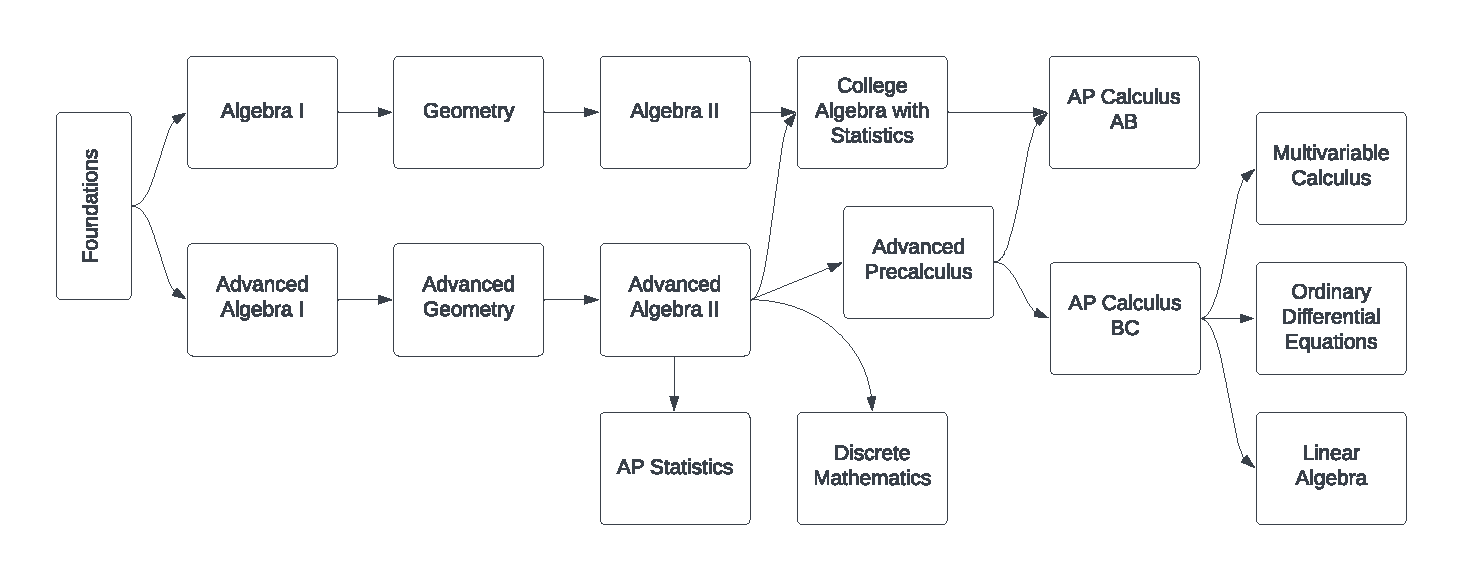
\includegraphics[scale=.5887]{prereq}  




\section{Course Descriptions}

\subsection{Current Courses}
\noindent\textbf{Foundations in Algebra and Geometry} \hfill TBD

\noindent Year - 1 Credit

\vspace{1mm}\emph{This first-year course prepares students for the challenges ahead in the math curriculum. Students examine and represent numbers in various forms; demonstrate fluency in mathematical language and understanding of concepts, processes, and reasoning; develop independence in learning mathematics; investigate math's scope and nature; and acquire a broad yet solid foundation for both algebra and geometry. They apply their learning to an array of problems.}\\

\noindent\textbf{Algebra I} \hfill TBD

\noindent Year - 1 Credit

\vspace{1mm}\emph{Algebra 1 is a course that introduces basic algebraic skills and focuses on problem solving techniques. It is designed as an introductory high school math course to provide a foundation for all subsequent math courses. Students must have a solid understanding pre-algebra topics, learn to think abstractly and become proficient problem solvers. Topics include, but are not limited to, properties of real numbers, relations and functions, linear equations and functions, Absolute value equations and functions, linear inequalities, systems of equations, properties of exponents, quadratic expressions and equations, radical expressions and equations, and rational expressions and equations. All units will contain graphical analysis, relating graphs to their corresponding expression or equation. The pace and depth of this course distinguishes it from Advance Algebra 1.}\\

\noindent\textbf{Advanced Algebra I} \hfill TBD

\noindent Year - 1 Credit

\vspace{1mm}\emph{Advanced Algebra 1 is a rigorous course that introduces basic algebraic skills and provides the foundation for all subsequent math courses. It is designed for students who have demonstrated exceptional ability and motivation in mathematics. Students must be highly motivated with a solid understanding pre-algebra topics, be able to think abstractly and be proficient problem solvers. Topics include, but are not limited to, properties of real numbers, relations and functions, linear equations and functions, Absolute value equations and functions, linear inequalities, systems of equations, properties of exponents, quadratic expressions and equations, radical expressions and equations, and rational expressions and equations. All units will contain graphical analysis, relating graphs to their corresponding expression or equation.}\\

\noindent\textbf{Geometry} \hfill TBD

\noindent Year - 1 Credit

\vspace{1mm}\emph{Geometry is a foundational course focused on the geometry of shapes, planes and space. Emphasis is placed on understanding, applying, justifying, and developing geometric properties in two and three dimensions. Students will engage in an in depth study of geometric reasoning, coordinate geometry, parallel and perpendicular lines, triangles, quadrilaterals, properties of polygons and circles, congruence and similarity, constructions, right triangle trigonometry, area, and volume. Students will apply this learning to solve real-world mathematical problems. The pace and depth of this course distinguishes it from Advanced Geometry.}\\

\noindent\textbf{Advanced Geometry} \hfill TBD

\noindent Year - 1 Credit

\vspace{1mm}\emph{Advanced Geometry is a foundational course focused on the geometry of shapes, planes and space. Emphasis is placed on understanding, applying, justifying, and developing geometric properties in two and three dimensions. Students will engage in an in depth study of geometric reasoning, coordinate geometry, parallel and perpendicular lines, triangles, quadrilaterals, properties of polygons and circles, congruence and similarity, constructions, right triangle trigonometry, area, and volume. Students will apply this learning to solve real-world mathematical problems.}\\

\noindent\textbf{Algebra II w/ Trigonometry} \hfill TBD

\noindent Year - 1 Credit

\vspace{1mm}\emph{Algebra II with Trigonometry is designed for students who have progressed the typical sequence of mathematics. It introduces students to advanced functions, with a focus on developing a strong conceptual grasp of the expressions that define them. Students learn through discovery and application, developing the skills they need to break down complex challenges and demonstrate their knowledge in new situations. To be successful students must complete daily work and be disciplined to read, listen, and think independently. Course topics include, but are not limited to, a complete study of function including quadratic functions, polynomial functions, rational functions, radical functions, exponential and logarithmic functions, and trigonometric functions. The pace and depth of this course distinguishes it from Advance Algebra 2.}\\

\noindent\textbf{Advanced Algebra II w/ Trigonometry} \hfill Thomas

\noindent Year - 1 Credit

\vspace{1mm}\emph{Advanced Algebra II with Trigonometry is designed for students who have demonstrated exceptional ability and motivation in mathematics. It introduces students to advanced functions, with a focus on developing a strong conceptual grasp of the expressions that define them. Students learn through discovery and application, developing the skills they need to break down complex challenges and demonstrate their knowledge in new situations. Students must be highly motivated with a solid understanding of previous math courses, be able to think abstractly and be proficient problem solvers. There is a rapid progression of topics and students must be able to perform within time limits. To be successful students must complete daily work and be disciplined to read, listen, and think independently. Course topics include, but are not limited to, a complete study of function including quadratic functions, polynomial functions, rational functions, radical functions, exponential and logarithmic functions, and trigonometric functions.}\\

\noindent\textbf{College Algebra with Statistics} \hfill TBD

\noindent Year - 1 Credit

\vspace{1mm}\emph{College Algebra and Statistics is a year-long course and is equivalent to an introductory college math course. This course is a functional approach to algebra that incorporates the use of appropriate technology. Emphasis will be placed on the study of functions and inequalities, including their graphs. Functions to be studied are linear, quadratic, piece-wise defined, absolute value, rational, polynomial, radical, exponential, logarithmic, and trigonometric functions. Appropriate applications will be included. In addition, this course will introduce students to the study of Statistics. Topics from Statistics to be covered are, but not limited to, numerical and graphical data analysis, probability, the Normal, Binomial, and Geometric Distributions, and simple linear regression.}\\

\noindent\textbf{Advanced Precalculus} \hfill TBD

\noindent Year - 1 Credit

\vspace{1mm}\emph{Advanced Precalculus is designed for the student who has a high interest in math or areas related to math. It builds on and completes the advanced concepts began in Advanced Algebra 1, Advanced Geometry and Advanced Algebra 2. Topics include, but are not limited to, polynomial and rational functions, complex numbers, determinants, inverse functions, trigonometry, logarithms, and exponentials. It introduces vectors, polar coordinates, parametric equations, matrix theory, partial fractions, limits, and some basic operations of calculus. }\\

\noindent\textbf{AP Calculus AB} \hfill TBD

\noindent Year - 1 Credit

\vspace{1mm}\emph{AP Calculus AB focuses on students’ understanding of calculus concepts and provides experience with methods and applications. Through the use of big ideas of calculus (e.g., modeling change, approximation and limits, and analysis of functions), the course becomes a cohesive whole, rather than a collection of unrelated topics. The course requires students to use definitions and theorems to build arguments and justify conclusions. The course features a multirepresentational approach to calculus, with concepts, results, and problems expressed graphically, numerically, analytically, and verbally. Exploring connections among these representations builds understanding of how calculus applies limits to develop important ideas, definitions, formulas, and theorems. A sustained emphasis on clear communication of methods, reasoning, justifications, and conclusions is essential. Teachers and students should regularly use technology to reinforce relationships among functions, to confirm written work, to implement experimentation, and to assist in interpreting results. This course follows the syllabus of the Advanced Placement Calculus AB exam. It is equivalent to one semester of college Calculus.}\\

\noindent\textbf{AP Statistics} \hfill Mullinax

\noindent Year - 1 Credit

\vspace{1mm}\emph{The AP Statistics course introduces students to the major concepts and tools for collecting, analyzing, and drawing conclusions from data. There are four themes evident in the content, skills, and assessment in the AP Statistics course: exploring data, sampling and experimentation, probability and simulation, and statistical inference. Students use technology, investigations, problem solving, and writing as they build conceptual understanding. This course follows the syllabus of the Advanced Placement Statistics Exam. This course is equivalent to an introductory Statistics in college.}\\

\noindent\textbf{AP Calculus BC} \hfill Mullinax

\noindent Year - 1 Credit

\vspace{1mm}\emph{AP Calculus BC focuses on students’ understanding of calculus concepts and provides experience with methods and applications. Through the use of big ideas of calculus (e.g., modeling change, approximation and limits, and analysis of functions), the course becomes a cohesive whole, rather than a collection of unrelated topics. The course requires students to use definitions and theorems to build arguments and justify conclusions. The course features a multirepresentational approach to calculus, with concepts, results, and problems expressed graphically, numerically, analytically, and verbally. Exploring connections among these representations builds understanding of how calculus applies limits to develop important ideas, definitions, formulas, and theorems. A sustained emphasis on clear communication of methods, reasoning, justifications, and conclusions is essential. Teachers and students should regularly use technology to reinforce relationships among functions, to confirm written work, to implement experimentation, and to assist in interpreting results. This course follows the syllabus of the Advanced Placement Calculus BC exam. It is equivalent to two semesters of college Calculus.}\\

\noindent\textbf{Differential Equations} \hfill LaCasse

\noindent Fall Semester - 0.5 Credits

\vspace{1mm}\emph{Introduces ordinary differential equations by means of algebraic, numerical, and graphical analysis (including phase-plane analysis). Examines first order differential equations, second and higher order linear equations, methods for nonhomogeneous second order equations, series solutions, Laplace transforms, linear systems, and linearization of nonlinear systems. Covers various applications throughout the course. Requires a graphing calculator with the TI-84 Plus series recommended. Students in this course will use the skills learned in calculus extensively. AP Calculus BC is a prerequisite.}\\

\noindent\textbf{Discrete \& Combinatorial Math} \hfill Gray

\noindent Spring Semester - 0.5 Credits

\vspace{1mm}\emph{One could say discrete mathematics is the study of the properties of the integers. In recent times, the importance of the field has been proven because computers work in a discrete manner (bits) and various mathematical structures can be used to represent theoretical models in computer science. In this course we will meander through various topics in discrete mathematics and step outside the standard curriculum to study knot theory (classification, invariants, knot polynomials). The standard curriculum will include set theory (naive, functions, injectivity, surjectivity, enumerating functions), combinatorics (permutations, combinations, complementary counting, symmetry, combinatorial proofs, 12-fold way), sequences (arithmetic/geometric sequences/sums, polynomial fitting, recurrence relations, characteristic root technique, induction), calculus of finite differences (factorial polynomials, fundamental theorem, antidifferences), number theory and group theory (divisibility, modular arithmetic, equations in Z/nZ, structure of Z/nZ for n prime, Chinese remainder theo- rem), graph theory (planarity, coloring, paths, circuits, bipartite graphs, incidence matrices), and apportionment.}\\

\noindent\textbf{Linear Algebra} \hfill Gray

\noindent Fall Semester - 0.5 Credits

\vspace{1mm}\emph{A standard treatment of linear algebra as presented to university-level mathematics majors. Course topics will include row-reduction, matrix equations, linear transformations, matrix opera- tions, invertibility, LU-factorization, subspaces of Euclidean space, dimension, rank, determinants (elementary product definition, expansion by minors, and row-reduction), vector spaces, null and column spaces, linear independence, bases, change of basis, eigen-theory, algebraic and geometric multiplicity, diagonalization, inner product, length, orthogonality, orthogonal sets, projections, the Gram-Schmidt process, QR-factorization, and the method least-squares.}\\

\noindent\textbf{Multivariable Calculus} \hfill LaCasse

\noindent Spring Semester - 0.5 Credits

\vspace{1mm}\emph{Multivariable Calculus is a college-level course that follows Advanced Placement Calculus BC. The course emphasizes a thorough study of vectors, surfaces in space, vector-valued functions, functions of several variables, multiple integrations, and vector analysis. Students will become proficient at vector operations including the dot product and cross product and their applications, rectangular coordinates, cylindrical coordinates, and spherical coordinates. Students will learn operations and applications of vector-valued functions including differentiation, integration, velocity, acceleration, tangent vectors, and normal vectors. Realizing that many real-life quantities are functions of two more variables, students will understand the following implementations of functions of several variables: limits, continuity, derivatives, and integration. The goal is to learn, understand, and be able to work with the main ideas of multivariable calculus.}\\



\chapter{Physical Education}

\section{Portrait of a Graduate}

\textsc{An Indian Springs School graduate, having completed the course of study in Physical Education, will} $\ldots$ 
\section{Course Descriptions}

\subsection{Current Courses}
\noindent\textbf{8th Grade PE} \hfill Pino/Skiff/Van Horn

\noindent Year - 1 Credit

\vspace{1mm}\emph{Students in 8th grade PE will have the opportunity to experience physical activity in a fun and safe manner.  Putting the body “in motion” is important to good physical health and can be a great stress release when dealing with the demands of a school day.  The goals of the course are to have the students be physically active, to learn new activities and skills, and to build self confidence in the students.}\\

\noindent\textbf{9th Grade PE} \hfill Pino

\noindent Spring Semester - 0.5 Credits

\vspace{1mm}\emph{Students will take what they have learned in Wellness and Fitness and implement that knowledge into their daily activities.  The focus will be working towards personal fitness goals through group and individual activities.}\\

\noindent\textbf{Well/Fit} \hfill Pino

\noindent Fall Semester - 0.5 Credits

\vspace{1mm}\emph{Wellness and Fitness is an introductory course dedicated to promoting a lifestyle which results in total health and wellness. The course is composed of both classroom and gym days consisting of personal assessment, taking notes, and physical activity.  Popular topics discussed include cardiovascular and muscular strength exercise, nutrition, and stress management.}\\

\noindent\textbf{Foundation of Sports Medicine and Safety} \hfill Skiff

\noindent Fall Semester - 0.5 Credits

\vspace{1mm}\emph{This course is designed to introduce the ideas and concepts that surround the growing field of sports medicine.  Students will explore the relationship of risk management and injury prevention through those fields that are defined as sports medicine. Students will examine the sports medicine team, sports medicine facilities, policies, procedures, and protocols utilized in patient care. Emphasis will be placed on health promotion, athlete wellness, and injury and disease prevention within athletic groups. Weekly discussions on current injured athletes will be highlighted.  This is a prerequisite to Sports Medicine I.}\\

\noindent\textbf{Injury Prevention \& Weight Training} \hfill Skiff

\noindent Fall and Spring Semesters - 0.5 Credits

\vspace{1mm}\emph{This course is designed to introduce the ideas and concepts that surround the prevention of injuries utilizing sound principles of weight training.  Students will learn the fundamentals of body assessment, establishing a physical foundation, and how to design a basic weight training/conditioning program specific to their needs.  Students will be able to identify general anatomy, weight room safety, correct weight lifting techniques, setting appropriate goals, yoga/stretching, and core work.}\\

\noindent\textbf{Sports Medicine} \hfill Skiff

\noindent Spring Semester - 0.5 Credits

\vspace{1mm}\emph{After establishing the basic understanding of the sports medicine team in Foundations of Sports Medicine and Safety, students will take a comprehensive look at the upper and lower extremities of the body.  Starting with the head and working their way down to the feet, the students will learn the anatomy, evaluation of the most common injuries, and basic rehabilitation of each body part.  Interactive labs will be introduced to include taking vitals, preventative taping, rehabilitation practices and the use of therapeutic modalities for the most common sports medicine injuries.}\\

\noindent\textbf{10th Grade PE} \hfill Van Horn

\noindent Year - 1 Credit

\vspace{1mm}\emph{Students in the 10th and 11th grade are required to find/develop a physical activity to meet their PE requirement of active exercise resulting in a minimum of 2-3 hours per week.  Physical activities may include any sport offered at Indian Springs School, other activities offered at Indian Springs School such as intramurals, or an outside-of-school program that involves physical exercise.  Any student-designed program must have a supervising instructor, meet two of the three components of fitness (cardiovascular endurance, muscular endurance and flexibility), and meet the approval of the PE department prior to the start of the program.}\\

\noindent\textbf{11th Grade PE} \hfill Van Horn

\noindent Year - 1 Credit

\vspace{1mm}\emph{Students in the 10th and 11th grade are required to find/develop a physical activity to meet their PE requirement of active exercise resulting in a minimum of 2-3 hours per week.  Physical activities may include any sport offered at Indian Springs School, other activities offered at Indian Springs School such as intramurals, or an outside-of-school program that involves physical exercise.  Any student-designed program must have a supervising instructor, meet two of the three components of fitness (cardiovascular endurance, muscular endurance and flexibility), and meet the approval of the PE department prior to the start of the program.}\\



\chapter{Science}

\section{Portrait of a Graduate}

\textsc{An Indian Springs School graduate, having completed the course of study in Science, will} $\ldots$ 

\begin{itemize}
  \item Engage in scientific questioning  to extend thinking and guide research.
\item Utilize experimental design and the scientific process to explore new ideas or solve problems.
\item Implement appropriate data collection techniques and analysis to interpret relevant scientific data versus biased data.
\item Evaluate scientific evidence to reach a valid conclusion.
\item Understand and appreciate the interconnectedness of the sciences.
\item Conduct literature reviews in order to incorporate other research into science writings.
\item Present research in front of a group of peers and defend research under questioning.
\item Apply appropriate mathematical principles and graphical analysis to solve problems and support ideas.
\item Utilize statistical tests and methods to accept or fail to accept scientific hypotheses.
\item Use the appropriate lab equipment, techniques, and technology when investigating scientific inquiries.
\item Use models and representations to communicate scientific phenomena and solve scientific problems.
\item Engage in problem solving, inquiry, and design of innovative solutions. 
\item Integrate prior knowledge with new information in novel and creative ways to strengthen overall understanding. 
\item Develop curiosity for the natural world with regard to scientific inquiry.
\item Apply conceptual understanding and critical thinking to real world problems.
\item Promote environmental stewardship.
\item Demonstrate the ability to collaborate with peers during scientific explorations.
\item Make a scientific claim and provide supportive evidence.
\item Connect the microscopic to the macroscopic across scientific disciplines.

\end{itemize}
\section{Course Descriptions}

\chapter{Individualized Learning}


\section{A Sample of Past Independent Studies}

\noindent{American Sign Language}

\noindent{Korean Language \& Culture}

\noindent{Game Theory}

\noindent{Cryptological Mathematics}

\noindent{Complex Variables}

\noindent{Mathematics of Finance}

\noindent{Demography}

\noindent{Tensegrity Structures}

\noindent{Statistical Analysis of Tennis}

\noindent{Abstract Algebra I \& II}

\noindent{Elementary Number Theory}

\noindent{Stock Markert Analysis}

\noindent{Adv. Chemical Techniques}

\noindent{Corvidology Study}

\noindent{History of Cosmology}

\noindent{A Survey of Modern Physics}

\noindent{Astrology}

\noindent{Canine Behavior \& Physiology}

\noindent{Anatomy \& Physiology of Domestic Animals}

\noindent{Geology}

\noindent{Nutrition Science}

\noindent{Nigerian Ind. \& Yoruba Studies}

\noindent{Investment Strategy}

\noindent{History of Feminist Art}

\noindent{Historical Foundations of US Government}

\noindent{American Political Philosophy: Founders and Origins}

\noindent{The Russian Revolution}

\noindent{The Impact of the Washington Consensus on the Post-2007 World Economies}

\noindent{American Folk Music of the 19th Century}

\noindent{The Spanish Renaissance \& the Aftermath of the Reconquest}

\noindent{The Nietzscean Era of Philosophy}

\noindent{Fashion and its Relation to Women's Rights}

\noindent{Modern Adaptations of Greek Mythology}

\noindent{Imperial Japan}

\noindent{Existential Philosophy}

\noindent{Military History}

\noindent{Cultural Economic Theory}

\noindent{Jazz Harmony and Improvisation}

\noindent{A Conductor's Guide to BWV 71}

\noindent{Fashion Design}

\noindent{Exploring Expressionism}

\noindent{Interior Design}

\noindent{Anatomical Art}

\noindent{Animation Illustration}

\noindent{Hand Drawn Animation}

\noindent{Photography of Social Issues}

\noindent{20th Century Music Theory \& Practice}

\noindent{Explorative Drawing \& Mixed Media}

\noindent{Architectural Drawing}

\noindent{Fundamental Music Theory}

\noindent{Musical Engineering}

\noindent{Exploring the Medium: Acrylic Painting}

\chapter{Malone Schools Online Network}


\section{The Program}
Springs is  excited and proud to be a member of the Malone Schools Online Network (\href{https://maloneschoolsonline.org/}{MSON}) and is the only member school in the state of Alabama.  Per their FAQ\footnote{\href{https://maloneschoolsonline.org/faq/}{Source}}

\begin{quote}
  The Malone Schools Online Network (MSON) expands academic opportunities for motivated, upper-level students by connecting them with inspiring teachers and peers across the country in real-time online seminars. MSON courses provide challenge beyond the standard curriculum while nurturing students’ intellectual curiosity, building their independence and time management skills, and fostering relationships across geographical divides. Beyond its classes, MSON draws on its vibrant community to help teachers and school leaders collaborate and innovate in their schools, charting new territory in learning.
\end{quote}

\noindent \textbf{Malone School Online Networks Course Policies}


Note that MSON online courses meet at a fixed time, typically twice per week.  Because they do not fit into our rotating schedule, students will regularly miss their scheduled classes while attending their MSON course. 

\begin{enumerate}\itemsep=0mm
\item You must be a junior or senior to enroll.
\item The average from your core courses (English, History, Science, Math, Languages) from the “Quarter 3 - Report” must be at least 90.
\item You must have a good attendance record. 
\item The MSON course cannot be taken in place of an identical, or almost identical, course offered by the school, assuming the school course can be made to fit into your schedule. 
\item The course must be your 6th class (not counting PE in 11th grade). 
\item The course must be taken for credit. 
\item You must comply with the advertised add/drop dates, course prerequisites and the attendance and homework policies of the MSON instructor. 
\item You are responsible for catching up work that you miss from a Springs course because of your attendance at an MSON course.  \emph{This includes notifying your teacher at Springs ahead of every missed class.}  
\item Per MSON policy, their courses must be prioritized over all other courses/obligations.  This means you may have classes during a school break/holidays, other classes, choir, sports, and so on.  
\end{enumerate}

The MSON enrollment form can be found in Appendix 12.4.4



\chapter{Appendix}

\section{Special Dates}

\section{Daily Schedule}

\section{Special Schedules}

\subsection{45 Minute Activity Period}

\subsection{60 Minute Activity Period}

\section{Forms}

\subsection{Academic Overload Form}

\subsection{Departmental Overload Form}

\subsection{Non-Springs AP Exam Request}



\section{Sample Academic Paths}

\section{FAQ}







% *****************************************************************
% Backmatter
%******************************************************************

%\printindex

\end{document}

